\level{1}{Test}
	In questa appendice vengono riportati i test di accettazione, sistema, integrazione ed unità previsti.\\
	Per la descrizione dei diversi tipi di test e della sintassi utilizzata per indicarli si rimanda alla sezione Test del documento \insdoc{Norme di Progetto v6.00}.
	\level{2}{Test di accettazione}
	\level{3}{TA1}Lo sviluppatore deve verificare che sia possibile creare grafici tramite le API interne.
	 
		Allo sviluppatore è richiesto di
		\begin{itemize}
			\item scegliere il tipo di grafico che vuole creare;
			\item inserire i valori del grafico;
			\item inserire le impostazioni del grafico;
			\item verificare che venga creato il tipo di grafico desiderato.
		\end{itemize}

	\level{3}{TA1.1}Lo sviluppatore deve verificare che sia possibile creare un bar chart.

		Allo sviluppatore è richiesto di
		\begin{itemize}
			\item scegliere come tipo di grafico il bar chart;
			\item inserire i valori del grafico.
		\end{itemize}

	\level{3}{TA1.2}Lo sviluppatore deve verificare che sia possibile creare un line chart.

		Allo sviluppatore è richiesto di
		\begin{itemize}
			\item scegliere come tipo di grafico il line chart;
			\item inserire i valori del grafico.
		\end{itemize}

	\level{3}{TA1.3}Lo sviluppatore deve verificare che sia possibile creare un map chart.

		Allo sviluppatore è richiesto di
		\begin{itemize}
			\item scegliere come tipo di grafico il map chart;
			\item inserire i valori del grafico.
		\end{itemize}

	\level{3}{TA1.4}Lo sviluppatore deve verificare che sia possibile creare una table.

		Allo sviluppatore è richiesto di
		\begin{itemize}
			\item scegliere come tipo di grafico la table;
			\item inserire i valori del grafico.
		\end{itemize}

	\level{3}{TA1.5/1}Lo sviluppatore deve verificare che sia possibile scegliere delle impostazioni di un bar chart.

		Allo sviluppatore è richiesto di
		\begin{itemize}
			\item scegliere come tipo di grafico il bar chart;
			\item inserire delle impostazioni.
		\end{itemize}

	\level{3}{TA1.5/2}Lo sviluppatore deve verificare che sia possibile scegliere delle impostazioni di un line chart.

		Allo sviluppatore è richiesto di
		\begin{itemize}
			\item scegliere come tipo di grafico il line chart;
			\item inserire delle impostazioni.
		\end{itemize}

	\level{3}{TA1.5/3}Lo sviluppatore deve verificare che sia possibile scegliere delle impostazioni di un map chart.

		Allo sviluppatore è richiesto di
		\begin{itemize}
			\item scegliere come tipo di grafico il map chart;
			\item inserire delle impostazioni.
		\end{itemize}

	\level{3}{TA1.5/4}Lo sviluppatore deve verificare che sia possibile scegliere delle impostazioni di una table.

		Allo sviluppatore è richiesto di
		\begin{itemize}
			\item scegliere come tipo di grafico una table;
			\item inserire delle impostazioni.
		\end{itemize}

	\level{3}{TA1.5.1}Lo sviluppatore deve verificare che sia possibile scegliere le impostazioni riguardanti la legenda di un line chart.

		Allo sviluppatore è richiesto di
		\begin{itemize}
			\item scegliere come tipo di grafico il line chart;
			\item inserire le impostazioni riguardanti la legenda.
		\end{itemize}

	\level{3}{TA1.5.1.1}Lo sviluppatore deve verificare che sia possibile scegliere se visualizzare o nascondere la legenda di un line chart.
			
		Allo sviluppatore è richiesto di
		\begin{itemize}
			\item scegliere come tipo di grafico il line chart;
			\item inserire i valori del grafico;
			\item verificare che, selezionando l'impostazione per la visualizzazione della legenda line chart, la legenda venga visualizzata;
			\item verificare che, selezionando l'impostazione per la non visualizzare la legenda line chart, la legenda non venga visualizzata.
		\end{itemize}

	\level{3}{TA1.5.1.2}Lo sviluppatore deve verificare che sia possibile scegliere la posizione in cui visualizzare la legenda di un line chart.
			
		Allo sviluppatore è richiesto di
		\begin{itemize}
			\item scegliere come tipo di grafico il line chart;
			\item inserire i valori del grafico;
			\item selezionare l'impostazione per la visualuzzare il line chart;
			\item impostare la posizione in cui la leggenda del line chart deve essere visualizzata.

		\end{itemize}

	\level{3}{TA1.5.2}Lo sviluppatore deve verificare che sia possibile scegliere le impostazioni riguardanti la legenda di un bar chart.

		Allo sviluppatore è richiesto di
		\begin{itemize}
			\item scegliere come tipo di grafico il bar chart;
			\item inserire le impostazioni riguardanti la legenda.
		\end{itemize}

	\level{3}{TA1.5.2.1}Lo sviluppatore deve verificare che sia possibile scegliere se visualizzare o nascondere la legenda di un bar chart.
		
		Allo sviluppatore è richiesto di
		\begin{itemize}
			\item scegliere come tipo di grafico il bar chart;
			\item inserire i valori del grafico;
			\item verificare che, selezionando l'impostazione per la visualizzazione della legenda bar chart, la legenda venga visualizzata;
			\item verificare che, selezionando l'impostazione per la non visualizzare la legenda bar chart, la legenda non venga visualizzata.
		\end{itemize}

	\level{3}{TA1.5.2.2}Lo sviluppatore deve verificare che sia possibile scegliere la posizione in cui visualizzare la legenda di un bar chart.
			
		Allo sviluppatore è richiesto di
		\begin{itemize}
			\item scegliere come tipo di grafico il bar chart;
			\item inserire i valori del grafico;
			\item selezionare l'impostazione per la visualuzzare il line chart;
			\item impostare la posizione in cui la leggenda del line chart deve essere visualizzata.
		\end{itemize}

	\level{3}{TA1.5.3}Lo sviluppatore deve verificare che sia possibile scegliere le impostazioni riguardanti la legenda di un map chart.

		Allo sviluppatore è richiesto di
		\begin{itemize}
			\item scegliere come tipo di grafico il map chart;
			\item inserire le impostazioni riguardanti la legenda.
		\end{itemize}

	\level{3}{TA1.5.3.1}Lo sviluppatore deve verificare che sia possibile scegliere se visualizzare o nascondere la legenda di un map chart.
			
		Allo sviluppatore è richiesto di
		\begin{itemize}
			\item scegliere come tipo di grafico il map chart;
			\item inserire i valori del grafico;
			\item verificare che, selezionando l'impostazione per la visualizzazione della legenda map chart, la legenda venga visualizzata;
			\item verificare che, selezionando l'impostazione per la non visualizzare la legenda map chart, la legenda non venga visualizzata.
		\end{itemize}

	\level{3}{TA1.5.3.2}Lo sviluppatore deve verificare che sia possibile scegliere la posizione in cui visualizzare la legenda di un map chart.
			
		Allo sviluppatore è richiesto di
		\begin{itemize}
			\item scegliere come tipo di grafico il map chart;
			\item inserire i valori del grafico;
			\item selezionare l'impostazione per la visualuzzare il line chart;
			\item impostare la posizione in cui la leggenda del line chart deve essere visualizzata.
		\end{itemize}

	\level{3}{TA1.5.4/1}Lo sviluppatore deve verificare se è possibile inserire una descrizione testuale per un un bar chart.

		Allo sviluppatore è richiesto di
		\begin{itemize}
			\item scegliere come tipo di grafico il bar chart;
			\item inserire i valori del grafico; (forse non necessario perchè dovrebbe esser visualizzata indipendentemente)
			\item inserire una descrizione testuale del grafico.
		\end{itemize}

	\level{3}{TA1.5.4/2}Lo sviluppatore deve verificare se è possibile inserire una descrizione testuale per un line chart.

		Allo sviluppatore è richiesto di
		\begin{itemize}
			\item scegliere come tipo di grafico il line chart;
			\item inserire i valori del grafico; (forse non necessario perchè dovrebbe esser visualizzata indipendentemente)
			\item inserire una descrizione testuale del grafico.
		\end{itemize}

	\level{3}{TA1.5.4/3}Lo sviluppatore deve verificare se è possibile inserire una descrizione testuale per un map chart.

		Allo sviluppatore è richiesto di
		\begin{itemize}
			\item scegliere come tipo di grafico il map chart;
			\item inserire i valori del grafico; (forse non necessario perchè dovrebbe esser visualizzata indipendentemente)
			\item inserire una descrizione testuale del grafico.
		\end{itemize}

	\level{3}{TA1.5.4/4}Lo sviluppatore deve verificare se è possibile inserire una descrizione testuale per in una table.

		Allo sviluppatore è richiesto di
		\begin{itemize}
			\item scegliere come tipo di grafico la table;
			\item inserire i valori del grafico; (forse non necessario perchè dovrebbe esser visualizzata indipendentemente)
			\item inserire una descrizione testuale del grafico.
		\end{itemize}

	\level{3}{TA1.5.5}Lo sviluppatore deve verificare che sia possibile scegliere le impostazioni riguardanti il piano cartesiano di un line chart.

		Allo sviluppatore è richiesto di
		\begin{itemize}
			\item scegliere come tipo di grafico il line chart;
			\item inserire le impostazioni riguardanti il piano cartesiano.
		\end{itemize}

	\level{3}{TA1.5.5.1}Lo sviluppatore deve verificare se è possibile inserire il nome dei due assi cartesiani di un line chart.

		Allo sviluppatore è richiesto di
		\begin{itemize}
			\item scegliere come tipo di grafico il line chart;
			\item inserire i valori del grafico;
			\item inserire il nome dei due assi cartesiani.
		\end{itemize}

	\level{3}{TA1.5.5.2}Lo sviluppatore deve verificare se è possibile scegliere se le linee della griglia di un line chart sono visualizzate o nascoste.

		Allo sviluppatore è richiesto di:
		\begin{itemize}
			\item scegliere come tipo di grafico il line chart;
			\item inserire i valori del grafico;
			\item scegliere se le linee della griglia sono visualizzate o nascoste.
		\end{itemize}

	\level{3}{TA1.5.6}Lo sviluppatore deve verificare che sia possibile scegliere le impostazioni riguardanti il piano cartesiano di un bar chart.

		Allo sviluppatore è richiesto di
		\begin{itemize}
			\item scegliere come tipo di grafico il bar chart;
			\item inserire le impostazioni riguardanti il piano cartesiano.
		\end{itemize}

	\level{3}{TA1.5.6.1}Lo sviluppatore deve verificare se è possibile inserire il nome dei due assi cartesiani di un bar chart.

		Allo sviluppatore è richiesto di
		\begin{itemize}
			\item scegliere come tipo di grafico il bar chart;
			\item inserire i valori del grafico;
			\item scegliere il massimo numero di dati visualizzati per ogni serie.
		\end{itemize}

	\level{3}{TA1.5.6.2}Lo sviluppatore deve verificare se è possibile scegliere se le linee della griglia di un bar chart sono visualizzate o nascoste.

		Allo sviluppatore è richiesto di
		\begin{itemize}
			\item scegliere come tipo di grafico il bar chart;
			\item inserire i valori del grafico;
			\item scegliere se le linee della griglia sono visualizzate o nascoste.
		\end{itemize}

	\level{3}{TA1.5.7/1}Lo sviluppatore deve verificare che sia possibile scegliere le impostazioni per scegliere il formato di stampa dei dati di un bar chart.

		Allo sviluppatore è richiesto di
		\begin{itemize}
			\item scegliere come tipo di grafico il bar chart;
			\item inserire le impostazioni per scegliere il formato di stampa dei dati.
		\end{itemize}

	\level{3}{TA1.5.7/2}Lo sviluppatore deve verificare che sia possibile scegliere le impostazioni per scegliere il formato di stampa dei dati di un line chart.

		Allo sviluppatore è richiesto di
		\begin{itemize}
			\item scegliere come tipo di grafico il line chart;
			\item inserire le impostazioni per scegliere il formato di stampa dei dati.
		\end{itemize}

	\level{3}{TA1.5.7/3}Lo sviluppatore deve verificare che sia possibile scegliere le impostazioni per scegliere il formato di stampa dei dati di un map chart.

		Allo sviluppatore è richiesto di
		\begin{itemize}
			\item scegliere come tipo di grafico il map chart;
			\item inserire le impostazioni per scegliere il formato di stampa dei dati.
		\end{itemize}

	\level{3}{TA1.5.7/4}Lo sviluppatore deve verificare che sia possibile scegliere le impostazioni per scegliere il formato di stampa dei dati di una table.

		Allo sviluppatore è richiesto di
		\begin{itemize}
			\item scegliere come tipo di grafico la table;
			\item inserire le impostazioni per scegliere il formato di stampa dei dati.
		\end{itemize}

	\level{3}{TA1.5.7.1}Lo sviluppatore deve verificare se è possibile impostare il colore del testo di ogni cella in una table.

		Allo sviluppatore è richiesto di
		\begin{itemize}
			\item scegliere come tipo di grafico la table;
			\item inserire i valori del grafico;
			\item impostare il colore del testo di ogni cella.
		\end{itemize}

	\level{3}{TA1.5.7.2}Lo sviluppatore deve verificare se è possibile impostare il colore dello sfondo di ogni cella in una table.

		Allo sviluppatore è richiesto di
		\begin{itemize}
			\item scegliere come tipo di grafico la table;
			\item inserire i valori del grafico;
			\item impostare il colore dello sfondo di ogni cella.
		\end{itemize}

	\level{3}{TA1.5.7.3}Lo sviluppatore deve verificare se è possibile impostare la dimensione dello spazio tra due serie di un bar chart.

		Allo sviluppatore è richiesto di
		\begin{itemize}
			\item scegliere come tipo di grafico il bar chart;
			\item inserire i valori del grafico;
			\item impostare la dimensione dello spazio tra due serie.
		\end{itemize}

	\level{3}{TA1.5.7.4}Lo sviluppatore deve verificare se è possibile impostare la dimensione dello spazio tra due valori di un bar chart.

		Allo sviluppatore è richiesto di
		\begin{itemize}
			\item scegliere come tipo di grafico il bar chart;
			\item inserire i valori del grafico;
			\item impostare la dimensione dello spazio tra due serie.
		\end{itemize}

	\level{3}{TA1.5.7.5}Lo sviluppatore deve verificare se è possibile scegliere la forma dei marcatori del map chart.

		Allo sviluppatore è richiesto di
		\begin{itemize}
			\item scegliere come tipo di grafico il map chart;
			\item inserire i valori del grafico;
			\item scegliere la forma dei marcatori.
		\end{itemize}

	\level{3}{TA1.5.7.6}Lo sviluppatore deve verificare se è possibile impostare la dimensione dei punti nel line chart.

		Allo sviluppatore è richiesto di
		\begin{itemize}
			\item scegliere come tipo di grafico il line chart;
			\item inserire i valori del grafico;
			\item impostare la dimensione dei punti.
		\end{itemize}

	\level{3}{TA1.5.7.7}Lo sviluppatore deve verificare se è possibile scegliere se la linea di un line chart è curva o segmentata.

		Allo sviluppatore è richiesto di
		\begin{itemize}
			\item scegliere come tipo di grafico il line chart;
			\item inserire i valori del grafico;
			\item scegliere se la linea di un line chart è curva o segmentata.
		\end{itemize}

	\level{3}{TA1.5.8}Lo sviluppatore deve verificare se è possibile scegliere l'orientamento delle barre tra verticale e orizzontale in un bar chart.

		Allo sviluppatore è richiesto di
		\begin{itemize}
			\item scegliere come tipo di grafico il bar chart;
			\item inserire i valori del grafico;
			\item scegliere l'orientamento delle barre tra verticale e orizzontale.
		\end{itemize}

	\level{3}{TA1.5.9}Lo sviluppatore deve verificare se è possibile scegliere le dimensioni dell'area visualizzata in un map chart.

		Allo sviluppatore è richiesto di
		\begin{itemize}
			\item scegliere come tipo di grafico il map chart;
			\item inserire i valori del grafico;
			\item scegliere l'orientamento delle barre tra verticale e orizzontale.
		\end{itemize}

	\level{3}{TA1.5.10}Lo sviluppatore deve verificare se è possibile scegliere il punto centrale della mappa in un map chart.

		Allo sviluppatore è richiesto di
		\begin{itemize}
			\item scegliere come tipo di grafico il map chart;
			\item inserire i valori del grafico;
			\item scegliere il punto centrale della mappa.
		\end{itemize}

	\level{3}{TA1.5.11/1}Lo sviluppatore deve verificare se è possibile scegliere il massimo numero di dati visualizzati per ogni serie di un line chart.

		Allo sviluppatore è richiesto di
		\begin{itemize}
			\item scegliere come tipo di grafico il line chart;
			\item inserire i valori del grafico;
			\item scegliere il massimo numero di dati visualizzati per ogni serie.
		\end{itemize}

	\level{3}{TA1.5.11/2}Lo sviluppatore deve verificare se è possibile scegliere il massimo numero di dati visualizzati per ogni serie di un bar chart.

		Allo sviluppatore è richiesto di
		\begin{itemize}
			\item scegliere come tipo di grafico il bar chart;
			\item inserire i valori del grafico;
			\item scegliere il massimo numero di dati visualizzati per ogni serie.
		\end{itemize}

	\level{3}{TA1.5.11/3}Lo sviluppatore deve verificare se è possibile scegliere il massimo numero di dati visualizzati per ogni serie di un map chart.

		Allo sviluppatore è richiesto di
		\begin{itemize}
			\item scegliere come tipo di grafico il map chart;
			\item inserire i valori del grafico;
			\item scegliere il massimo numero di dati visualizzati per ogni serie.
		\end{itemize}

	\level{3}{TA1.5.12}Lo sviluppatore deve verificare se è possibile scegliere il massimo numero di righe visualizzate di una table.

		Allo sviluppatore è richiesto di
		\begin{itemize}
			\item scegliere come tipo di grafico una table;
			\item inserire i valori del grafico;
			\item scegliere il massimo numero di righe visualizzate.
		\end{itemize}

	\level{3}{TA1.5.13}Lo sviluppatore deve verificare se è possibile ordinare i dati per colonna in una table.

		Allo sviluppatore è richiesto di
		\begin{itemize}
			\item scegliere come tipo di grafico una table;
			\item inserire i valori del grafico;
			\item ordinare i dati per colonna.
		\end{itemize}

	\level{3}{TA1.5.14}Lo sviluppatore deve verificare se è possibile scegliere la posizione in cui vengono aggiunte nuove righe in una table.

		Allo sviluppatore è richiesto di
		\begin{itemize}
			\item scegliere come tipo di grafico una table;
			\item inserire i valori del grafico;
			\item scegliere la posizione in cui vengono aggiunte nuove righe.
		\end{itemize}

	\level{3}{TA1.5.15}Lo sviluppatore deve verificare se è possibile scegliere l'intestazione di ciascuna colonna in una table.

		Allo sviluppatore è richiesto di
		\begin{itemize}
			\item scegliere come tipo di grafico una table;
			\item inserire i valori del grafico;
			\item scegliere l'intestazione di ciascuna colonna.
		\end{itemize}

	\level{3}{TA1.5.16}Lo sviluppatore deve verificare se è possibile scegliere se le linee di una table sono visualizzate o nascoste.

		Allo sviluppatore è richiesto di
		\begin{itemize}
			\item scegliere come tipo di grafico una table;
			\item inserire i valori del grafico;
			\item scegliere se le linee sono visualizzate o nascoste.
		\end{itemize}

	\level{3}{TA1.5.17/1}Lo sviluppatore deve verificare se è possibile impostare il titolo in un bar chart.

		Allo sviluppatore è richiesto di
		\begin{itemize}
			\item scegliere come tipo di grafico il bar chart;
			\item impostare il titolo del grafico.
		\end{itemize}

	\level{3}{TA1.5.17/2}Lo sviluppatore deve verificare se è possibile impostare il titolo in un line chart.

		Allo sviluppatore è richiesto di
		\begin{itemize}
			\item scegliere come tipo di grafico il line chart;
			\item impostare il titolo del grafico.
		\end{itemize}

	\level{3}{TA1.5.17/3}Lo sviluppatore deve verificare se è possibile impostare il titolo in un map chart.

		Allo sviluppatore è richiesto di
		\begin{itemize}
			\item scegliere come tipo di grafico il map chart;
			\item impostare il titolo del grafico.
		\end{itemize}

	\level{3}{TA1.5.17/4}Lo sviluppatore deve verificare se è possibile impostare il titolo in una table.

		Allo sviluppatore è richiesto di
		\begin{itemize}
			\item scegliere come tipo di grafico la table;
			\item impostare il titolo del grafico.
		\end{itemize}

	\level{3}{TA1.5.18}Lo sviluppatore deve verificare se è possibile scegliere il colore per ciascun set di dati in un line chart.

		Allo sviluppatore è richiesto di
		\begin{itemize}
			\item scegliere come tipo di grafico il line chart;
			\item inserire i valori del grafico;
			\item scegliere il colore per ciascun set di dati.
		\end{itemize}

	\level{3}{TA1.5.19}Lo sviluppatore deve verificare se è possibile scegliere il colore per ciascun set di dati in un bar chart.

		Allo sviluppatore è richiesto di
		\begin{itemize}
			\item scegliere come tipo di grafico il bar chart;
			\item inserire i valori del grafico;
			\item scegliere il colore per ciascun set di dati.
		\end{itemize}

	\level{3}{TA1.5.20}Lo sviluppatore deve verificare se è possibile scegliere il colore per ciascun set di dati in un map chart.

		Allo sviluppatore è richiesto di
		\begin{itemize}
			\item scegliere come tipo di grafico il map chart;
			\item inserire i valori del grafico;
			\item scegliere il colore per ciascun set di dati.
		\end{itemize}

	\level{3}{TA1.5.21}Lo sviluppatore deve verificare se è possibile scegliere il nome per ciascun set di dati di un line chart.

		Allo sviluppatore è richiesto di
		\begin{itemize}
			\item scegliere come tipo di grafico il line chart;
			\item inserire i valori del grafico;
			\item impostare il titolo del grafico.
		\end{itemize}

	\level{3}{TA1.5.22}Lo sviluppatore deve verificare se è possibile scegliere il nome per ciascun set di dati di un bar chart.

		Allo sviluppatore è richiesto di
		\begin{itemize}
			\item scegliere come tipo di grafico il bar chart;
			\item inserire i valori del grafico;
			\item impostare il titolo del grafico.
		\end{itemize}

	\level{3}{TA1.5.23}Lo sviluppatore deve verificare se è possibile scegliere il nome per ciascun set di dati di un map chart.

		Allo sviluppatore è richiesto di
		\begin{itemize}
			\item scegliere come tipo di grafico il map chart;
			\item inserire i valori del grafico;
			\item impostare il titolo del grafico.
		\end{itemize}

	\level{3}{TA1.6/1}Lo sviluppatore deve verificare se è possibile inserire i dati in un bar chart.

		Allo sviluppatore è richiesto di
		\begin{itemize}
			\item scegliere come tipo di grafico il bar chart;
			\item inserire i valori del grafico.
		\end{itemize}	
			
	\level{3}{TA1.6/2}Lo sviluppatore deve verificare se è possibile inserire i dati in un line chart.

		Allo sviluppatore è richiesto di
		\begin{itemize}
			\item scegliere come tipo di grafico il line chart;
			\item inserire i valori del grafico.
		\end{itemize}	

	\level{3}{TA1.6/3}Lo sviluppatore deve verificare se è possibile inserire i dati in una table.

		Allo sviluppatore è richiesto di
		\begin{itemize}
			\item scegliere come tipo di grafico la table;
			\item inserire i valori del grafico.
		\end{itemize}	

	\level{3}{TA1.6/4}Lo sviluppatore deve verificare se è possibile inserire i dati in un map chart.

		Allo sviluppatore è richiesto di
		\begin{itemize}
			\item scegliere come tipo di grafico il map chart;
			\item inserire i valori del grafico.
		\end{itemize}

	\level{3}{TA1.7}Lo sviluppatore deve verificare se viene visualizzato un errore qualora i dati passati per l'aggiornamento di un grafico siano scorretti.

		Allo sviluppatore è richiesto di
		\begin{itemize}
			\item creare un grafico di tipo x (è necessario rifare questo test per ogni grafico di tipo x messo a disposizione dal framework);
			\item inserire i dati;
			\item aggiornare il grafico con un metodo permesso dal grafico  di tipo x passando dei valori non presenti (valore della serie dei dati o valore da sostituire) nell'istanza del grafico;
			\item verificare che sia ritornato una segnalazione di errore.
		\end{itemize}

	\level{3}{TA1.8}Lo sviluppatore deve verificare se viene visualizzato un errore qualora i dati passati per la creazione di un grafico siano scorretti.

		Allo sviluppatore è richiesto di
		\begin{itemize}
			\item creare un grafico di tipo x (è necessario rifare questo test per ogni grafico di tipo x messo a disposizione dal framework);
			\item inserire i dati delle impostazioni o dei valori scorretti;
			\item verificare che sia ritornato una segnalazione di errore.
		\end{itemize}

	\level{3}{TA1.9}Lo sviluppatore deve verificare se viene visualizzato un errore qualora si cerchi di inserire un grafico oltre il limite consentito dalla pagina.

		Allo sviluppatore è richiesto di
		\begin{itemize}
			\item creare una pagina con massimo x grafici;
			\item inserire x+1 grafici;
			\item verificare che sia ritornato una segnalazione di errore.
		\end{itemize}

	\level{3}{TA1.10}Lo sviluppatore deve verificare se viene visualizzato un errore qualora si cerchi di aggiornare un grafico con un tipo di aggiornamento da lui non permesso.

		Allo sviluppatore è richiesto di
		\begin{itemize}
			\item creare un grafico di tipo x (è necessario rifare questo test per ogni grafico di tipo x messo a disposizione dal framework);
			\item inserire i dati;
			\item effettuare gli aggiornamenti non permessi;
			\item verificare che sia ritornato una segnalazione di errore.
		\end{itemize}

	\level{3}{TA2}Lo sviluppatore deve verificare se sia permesso l'aggiornamento di un grafico tramite le API interne.
		
		Allo sviluppatore è richiesto di
		\begin{itemize}
			\item creare un grafico inserendo dei dati;
			\item verificare che sia permesso l'aggiornamento di un grafico tramite le API interne.
		\end{itemize}

	\level{3}{TA2.1}Lo sviluppatore deve verificare se sia permesso l'aggiornamento stream di un grafico line chart
		
		Allo sviluppatore è richiesto di
		\begin{itemize}
			\item creare un grafico line chart;
			\item verificare che sia permesso l'aggiornamento stream per il grafico creato.
		\end{itemize}

	\level{3}{TA2.2}Lo sviluppatore deve verificare se sia permesso l'aggiornamento di un grafico table.
		
		Allo sviluppatore è richiesto di
		\begin{itemize}
			\item creare un grafico table;
			\item verificare che sia permesso l'aggiornamento stream per il grafico creato.
		\end{itemize}

	\level{3}{TA2.3}Lo sviluppatore deve verificare se sia permesso l'aggiornamento movie di un grafico map chart.
		
		Allo sviluppatore è richiesto di
		\begin{itemize}
			\item creare un grafico map chart;
			\item verificare che sia permesso l'aggiornamento movie per il grafico creato.
		\end{itemize}

	\level{3}{TA2.4}Lo sviluppatore deve verificare se sia permesso l'aggiornamento in place di un grafico bar chart.
		
		Allo sviluppatore è richiesto di
		\begin{itemize}
			\item creare un grafico bar chart;
			\item verificare che sia permesso l'aggiornamento in place per il grafico creato.
		\end{itemize}

	\level{3}{TA2.5}Lo sviluppatore deve verificare se sia permesso l'aggiornamento in place di un grafico line chart.
		
		Allo sviluppatore è richiesto di
		\begin{itemize}
			\item creare un grafico line chart
			\item verificare che sia permesso l'aggiornamento in place per il grafico creato.
		\end{itemize}

	\level{3}{TA2.6}Lo sviluppatore deve verificare se sia permesso l'aggiornamento in place di un grafico map chart.
		
		Allo sviluppatore è richiesto di
		\begin{itemize}
			\item creare un grafico map chart
			\item verificare che sia permesso l'aggiornamento in place per il grafico creato.
		\end{itemize}

	\level{3}{TA2.7}Lo sviluppatore deve verificare se sia permesso l'aggiornamento in place di un grafico table.
		
		Allo sviluppatore è richiesto di
		\begin{itemize}
			\item creare un grafico table;
			\item verificare che sia permesso l'aggiornamento in place per il grafico creato.
		\end{itemize}

	\level{3}{TA3}Lo sviluppatore deve verificare se sia permessa la creazione di una pagina HTML contenente alcuni grafici tramite le API interne.
		
		Allo sviluppatore è richiesto di
		\begin{itemize}
			\item creare un'istanza di Norris;
			\item creare una pagina;
			\item creare un grafico da associare a quella pagina;
			\item aggiungere il grafico ala pagina.
		\end{itemize}

	\level{3}{TA3.1}Lo sviluppatore deve verificare se sia permesso l'inserimento del titolo nella pagina.
		
		Allo sviluppatore è richiesto di
		\begin{itemize}
			\item creare un'istanza di Norris;
			\item creare una pagina;
			\item impostare il titolo di quella pagina;
		\end{itemize}

	\level{3}{TA3.2}Lo sviluppatore deve verificare se sia permesso la scelta delle opzioni di visualizzazione.
		
		Allo sviluppatore è richiesto di
		\begin{itemize}
			\item creare un'istanza di Norris;
			\item creare una pagina;
			\item impostare l'opzione di visualizzazione desiderata per quella pagina.
		\end{itemize}

	\level{3}{TA3.2.1}Lo sviluppatore deve verificare se sia permessa l'impostazione del massimo numero di grafici nella pagina.
		
		Allo sviluppatore è richiesto di
		\begin{itemize}
			\item creare un'istanza di Norris;
			\item creare una pagina;
			\item impostare il massimo numero di grafici per quella pagina.
		\end{itemize}

	\level{3}{TA3.2.2}Lo sviluppatore deve verificare se sia permessa l'impostazione del massimo numero di grafici visualizzabile per colonna in una pagina.
		
		Allo sviluppatore è richiesto di
		\begin{itemize}
			\item creare un'istanza di Norris;
			\item creare una pagina;
			\item impostare l'opzione di visualizzazione;
			\item impostare il massimo numero di grafici visualizzabile per colonna in quella pagina;
		\end{itemize}

	\level{3}{TA3.3}Lo sviluppatore deve verificare se sia permesso l'aggiunta di grafici nella pagina.
		
		Allo sviluppatore è richiesto di
		\begin{itemize}
			\item creare un'istanza di Norris;
			\item creare una pagina;
			\item creare almeno un grafico;
			\item aggiungere i grafici creati alla pagina.
		\end{itemize}

	\level{3}{TA4}Lo sviluppatore deve verificare che il framework permetta di ottenere un middleware per Express.js tramite le API interne.
		
		Allo sviluppatore è richiesto di
		\begin{itemize}
			\item verificare che sia possibile ottenere un middleware per Express.js tramite le funzionlità offerte dalle API interne.
		\end{itemize}

	\level{3}{TA5}L'utente client deve verificare che il framework permetta di ottenere tramite le API esterne le informazioni sui grafici creati con le API interne.

		All'utente client è richiesto di
		\begin{itemize}
			\item autenticarsi ad una istanza di Norris esistente;
			\item verificare che, tramite le funzionalità offerte dalle API esterne, sia possibile ottenere le informazioni sui grafici esistenti.
		\end{itemize}

	\level{3}{TA5.1}L'utente client deve verificare che le API esterne permettano di ottenere la lista dei grafici presenti.

		All'utente client è richiesto di
		\begin{itemize}
			\item autenticarsi ad una istanza di Norris esistente;
			\item verificare che, tramite le funzionalità offerte dalle API esterne, sia possibile ottenere la lista dei grafici esistenti.
		\end{itemize}

	\level{3}{TA5.1.1}L'utente client deve verificare che la lista dei grafici fornisca ID, titolo, tipo e descrizione di ciascun grafico.
		
		All'utente client è richiesto di
		\begin{itemize}
			\item autenticarsi ad una istanza di Norris esistente;
			\item verificare che la lista dei grafici fornisca ID, titolo, tipo e descrizione di ciascun grafico.
		\end{itemize}

	\level{3}{TA5.2}L'utente client deve verificare che le API esterne permettano di ottenere i grafici con relativi aggiornamenti.
		
		All'utente client è richiesto di
		\begin{itemize}
			\item autenticarsi ad una istanza di Norris esistente;
			\item verificare che, tramite le funzionalità offerte dalle API esterne, sia possibile ottenere i grafici con relativi aggiornamenti.
		\end{itemize}

	\level{3}{TA5.3}L'utente client deve verificare che le API esterne permettano di accedere a un'istanza di Norris tramite username e password.
		
		All'utente client è richiesto di
		\begin{itemize}
			\item verificare che, tramite le funzionalità offerte dalle API esterne, sia possibile accedere a un'istanza di Norris tramite username e password.
		\end{itemize}

	\level{3}{TA5.4} L'utente client deve verificare che le API esterne permettano di scollegarsi  da un'istanza di Norris.
		
		All'utente client è richiesto di
		\begin{itemize}
			\item autenticarsi ad una istanza di Norris esistente;
			\item verificare che, tramite le funzionalità offerte dalle API esterne, sia possibile scollegarsi da un'istanza di Norris.
		\end{itemize}

	\level{3}{TA6}L'utente client deve verificare che il framework permetta l'inserimento di grafici all'interno di pagine HTML tramite un'apposita libreria .
		
		All'utente client è richiesto di
		\begin{itemize}
			\item autenticarsi ad una istanza di Norris esistente;
			\item verificare che, tramite le funzionalità offerte dalla libreria, sia possibile inserire grafici esistenti all'interno di pagine HTML.
		\end{itemize}

	\level{3}{TA6.1}L'utente client deve verificare che la libreria permetta l'inserimento di un grafico all'interno di un determinato tag HTML.
		
		All'utente client è richiesto di
		\begin{itemize}
			\item autenticarsi ad una istanza di Norris esistente;
			\item scegliere un grafico dell'istanza di Norris;
			\item verificare che, tramite le funzionalità offerte dalla libreria, sia possibile inserire il grafico scelto all'interno di un determinato tag HTML;
			\item ripetere la verifica per ogni grafico.
		\end{itemize}

	\level{3}{TA6.2}L'utente client deve verificare che la libreria permetta di modificare le principali impostazioni di un grafico.
		
		All'utente client è richiesto di
		\begin{itemize}
			\item autenticarsi ad una istanza di Norris esistente;
			\item scegliere un grafico dell'istanza di Norris;
			\item verificare che, tramite le funzionalità offerte dalla libreria, sia possibile modificare le principali impostazioni del grafico;
			\item ripetere la verifica per ogni grafico.
		\end{itemize}

	\level{3}{TA6.2.1}L'utente client deve verificare che la libreria permetta di modificare la scelta se visualizzare o meno la legenda di un line chart.
		
		All'utente client è richiesto di
		\begin{itemize}
			\item autenticarsi ad una istanza di Norris esistente;
			\item scegliere un grafico di tipo line chart dell'istanza di Norris;
			\item verificare che, tramite le funzionalità offerte dalla libreria, sia possibile modificare la scelta se visualizzare o meno la legenda di un line chart.
			\item ripetere la verifica per ogni grafico di tipo line chart.
		\end{itemize}

	\level{3}{TA6.2.2}L'utente client deve verificare che la libreria permetta di modificare la scelta se visualizzare o meno la legenda di un bar chart.
		
		All'utente client è richiesto di
		\begin{itemize}
			\item autenticarsi ad una istanza di Norris esistente;
			\item scegliere un grafico di tipo bar chart dell'istanza di Norris;
			\item verificare che, tramite le funzionalità offerte dalla libreria, sia possibile modificare la scelta se visualizzare o meno la legenda di un bar chart.
			\item ripetere la verifica per ogni grafico di tipo bar chart.
		\end{itemize}

	\level{3}{TA6.2.3}L'utente client deve verificare che la libreria permetta di modificare la scelta se visualizzare o meno la legenda di un map chart.
		
		All'utente client è richiesto di
		\begin{itemize}
			\item autenticarsi ad una istanza di Norris esistente;
			\item scegliere un grafico di tipo map chart dell'istanza di Norris;
			\item verificare che, tramite le funzionalità offerte dalla libreria, sia possibile modificare la scelta se visualizzare o meno la legenda di un map chart.
			\item ripetere la verifica per ogni grafico di tipo map chart.
		\end{itemize}

	\level{3}{TA6.2.4}L'utente client deve verificare che la libreria permetta di modificare la posizione in cui è visualizzata la legenda di un line chart.
		
		All'utente client è richiesto di
		\begin{itemize}
			\item autenticarsi ad un'istanza di Norris esistente;
			\item scegliere un grafico di tipo line chart dell'istanza di Norris;
			\item verificare che, tramite le funzionalità offerte dalla libreria, sia possibile modificare la posizione in cui è visualizzata la legenda di un line chart.
			\item ripetere la verifica per ogni grafico di tipo line chart.
		\end{itemize}

	\level{3}{TA6.2.5}L'utente client deve verificare che la libreria permetta di modificare la posizione in cui è visualizzata la legenda di un bar chart.
		
		All'utente client è richiesto di
		\begin{itemize}
			\item autenticarsi ad un'istanza di Norris esistente;
			\item scegliere un grafico di tipo bar chart dell'istanza di Norris;
			\item verificare che, tramite le funzionalità offerte dalla libreria, sia possibile modificare la posizione in cui è visualizzata la legenda di un bar chart.
			\item ripetere la verifica per ogni grafico di tipo bar chart.
		\end{itemize}

	\level{3}{TA6.2.6}L'utente client deve verificare che la libreria permetta di modificare la posizione in cui è visualizzata la legenda di un map chart.
		
		All'utente client è richiesto di
		\begin{itemize}
			\item autenticarsi ad un'istanza di Norris esistente;
			\item scegliere un grafico di tipo map chart dell'istanza di Norris;
			\item verificare che, tramite le funzionalità offerte dalla libreria, sia possibile modificare la posizione in cui è visualizzata la legenda di un map chart.
			\item ripetere la verifica per ogni grafico di tipo map chart.
		\end{itemize}

	\level{3}{TA6.2.7}L'utente client deve verificare che la libreria permetta di modificare la scelta se visualizzare o meno la griglia del piano cartesiano di un line chart.
		
		All'utente client è richiesto di
		\begin{itemize}
			\item autenticarsi ad un'istanza di Norris esistente;
			\item scegliere un grafico di tipo line chart dell'istanza di Norris;
			\item verificare che, tramite le funzionalità offerte dalla libreria, sia possibile modificare la scelta se visualizzare o meno la griglia del piano cartesiano di un line chart.
			\item ripetere la verifica per ogni grafico di tipo line chart.
		\end{itemize}

	\level{3}{TA6.2.8}L'utente client deve verificare che la libreria permetta di modificare la scelta se visualizzare o meno la griglia del piano cartesiano di un bar chart.
		
		All'utente client è richiesto di
		\begin{itemize}
			\item autenticarsi ad un'istanza di Norris esistente;
			\item scegliere un grafico di tipo bar chart dell'istanza di Norris;
			\item verificare che, tramite le funzionalità offerte dalla libreria, sia possibile modificare la scelta se visualizzare o meno la griglia del piano cartesiano di un bar chart.
			\item ripetere la verifica per ogni grafico di tipo bar chart.
		\end{itemize}

	\level{3}{TA6.2.9}L'utente client deve verificare che la libreria permetta di modificare il colore di ciascun set di dati di un line chart.
		
		All'utente client è richiesto di
		\begin{itemize}
			\item autenticarsi ad un'istanza di Norris esistente;
			\item scegliere un grafico di tipo line chart dell'istanza di Norris;
			\item verificare che, tramite le funzionalità offerte dalla libreria, sia possibile modificare il colore di ciascun set di dati di un line chart.
			\item ripetere la verifica per ogni grafico di tipo line chart.
		\end{itemize}

	\level{3}{TA6.2.10}L'utente client deve verificare che la libreria permetta di modificare il colore di ciascun set di dati di un bar chart.
		
		All'utente client è richiesto di
		\begin{itemize}
			\item autenticarsi ad un'istanza di Norris esistente;
			\item scegliere un grafico di tipo bar chart dell'istanza di Norris;
			\item verificare che, tramite le funzionalità offerte dalla libreria, sia possibile modificare il colore di ciascun set di dati di un bar chart.
			\item ripetere la verifica per ogni grafico di tipo line chart.
		\end{itemize}

	\level{3}{TA6.2.11}L'utente client deve verificare che la libreria permetta di modificare il colore di ciascun set di dati di un map chart.
		
		All'utente client è richiesto di
		\begin{itemize}
			\item autenticarsi ad un'istanza di Norris esistente;
			\item scegliere un grafico di tipo map chart dell'istanza di Norris;
			\item verificare che, tramite le funzionalità offerte dalla libreria, sia possibile modificare il colore di ciascun set di dati di un map chart.
			\item ripetere la verifica per ogni grafico di tipo map chart.
		\end{itemize}

	\level{3}{TA6.2.12}L'utente client deve verificare che la libreria permetta di modificare il colore di sfondo di ogni cella per la table.
		
		All'utente client è richiesto di
		\begin{itemize}
			\item autenticarsi ad un'istanza di Norris esistente;
			\item scegliere un grafico di tipo table dell'istanza di Norris;
			\item verificare che, tramite le funzionalità offerte dalla libreria, sia possibile modificare il colore di sfondo di ogni cella per la table.
			\item ripetere la verifica per ogni grafico di tipo table.
		\end{itemize}

	\level{3}{TA6.2.13}L'utente client deve verificare che la libreria permetta di modificare il colore del testo contenuto in ogni cella per la table.
		
		All'utente client è richiesto di
		\begin{itemize}
			\item autenticarsi ad un'istanza di Norris esistente;
			\item scegliere un grafico di tipo table dell'istanza di Norris;
			\item verificare che, tramite le funzionalità offerte dalla libreria, sia possibile modificare il colore del testo contenuto in ogni cella per la table.
			\item ripetere la verifica per ogni grafico di tipo table.
		\end{itemize}

	\level{3}{TA6.3}L'utente client deve verificare che la libreria CHUCK permetta di accedere a un'istanza di Norris tramite username e password.
		
		All'utente client è richiesto di
		\begin{itemize}
			\item verificare che, tramite le funzionalità offerte dalla libreria Chuck, sia possibile raggiungere un'istanza di Norris tramite username e password.
		\end{itemize}

	\level{3}{TA6.4}L'utente client deve verificare che la libreria CHUCK permetta di scollegarsi da un'istanza di Norris.

		All'utente client è richiesto di
		\begin{itemize}
			\item autenticarsi ad un'istanza di Norris esistente;
			\item verificare che, tramite le funzionalità offerte dalla libreria Chuck, sia possibile scollegarsi dall'istanza di Norris.
		\end{itemize}

	\level{3}{TA7}L'utente deve verificare che la dashboard permetta di visualizzare in tempo reali gli autobus dell'APS.

		All'utente è richiesto di
		\begin{itemize}
			\item andare all'indirizzo della dasborad;
			\item verificare che vengano mostrati gli autobus dell'APS;
			\item verificare che gli aggiornamenti avvengano in tempo reale, senza dover aggiornare la pagina.
		\end{itemize}

	\level{3}{TA7.1}L'utente deve verificare che la dashboard permetta di visualizzare il numero di autobus attivi per ciascuna linea.

		All'utente è richiesto di
		\begin{itemize}
			\item andare all'indirizzo della dasborad;
			\item verificare che vengano mostrati il numero di autobus attivi per ciascuna linea.
		\end{itemize}

	\level{3}{TA7.2}L'utente deve verificare che la dashboard permetta di filtrare gli autobus per linea di appartenenza e visualizzarli di conseguenza.

		All'utente è richiesto di
		\begin{itemize}
			\item andare all'indirizzo della dasborad;
			\item selezionare le linee che vogliono visualizzare;
			\item verificare che vengano mostrati solo gli autobus delle linee selezionate;
		\end{itemize}

	\level{3}{TA8}L'utente deve verificare che l'applicazione Android permetta di visualizzare dei grafici.

		All'utente è richiesto di
		\begin{itemize}
			\item installare l'apk;
			\item accedere ad una istanza di Norris;
			\item verificare che sia possibile visualizzare i grafici.
		\end{itemize}

	\level{3}{TA8.1}L'utente deve verificare che l'applicazione Android permetta di accedere a un'istanza di Norris tramite username e password.

		All'utente è richiesto di
		\begin{itemize}
			\item avviare l'applicazione;
			\item inserire l'indirizzo di un'istanza di Norris;
			\item inserire le credenziali di autenticazione;
			\item verificare che sia visualizzata la lista dei grafici presenti nell'istanza di Norris scelta.
		\end{itemize}

	\level{3}{TA8.2}L'utente deve verificare che l'applicazione Android permetta di visualizzare l'elenco dei grafici esistenti nell'istanza Norris con relativo ID, titolo, tipo e descrizione.

		All'utente è richiesto di
		\begin{itemize}
			\item avviare l'applicazione;
			\item inserire un indirizzo valido di un'istanza di Norris e se necessario autenticarsi;
			\item verificare che sia visualizzabile l'elenco dei grafici esistenti nell'istanza Norris con relativo ID, titolo, tipo e descrizione.
		\end{itemize}

	\level{3}{TA8.3}L'utente deve verificare che l'applicazione Android permetta di selezionare e visualizzare un singolo grafico dell'istanza di Norris.

		All'utente è richiesto di
		\begin{itemize}
			\item avviare l'applicazione;
			\item inserire un indirizzo valido di un'istanza di Norris ed autenticarsi se necessario;
			\item selezionare un grafico dalla lista di grafici presenti;
			\item verificare visivamente la presenza di un singolo grafico e che quel grafico sia quello selezinato.
		\end{itemize}

	\level{3}{TA8.4}L'utente deve verificare che l'applicazione Android mostri un errore quando viene immesso un indirizzo per un'istanza di Norris non valido.

		All'utente è richiesto di
		\begin{itemize}
			\item avviare l'applicazione;
			\item inserire un indirizzo per un'istanza di Norris non valido;
			\item verificare che venga segnalato un errore;
		\end{itemize}

	\level{3}{TA8.5}L'utente deve verificare che l'applicazione Android mostri un errore quando vengono immessi dati di accesso (username e password) per un'istanza di Norris non validi.

		All'utente è richiesto di
		\begin{itemize}
			\item avviare l'applicazione;
			\item inserire l'indirizzo di un'istanza di Norris;
			\item autenticarsi con credenziali errate;
			\item verificare che venga segnalato un errore di autenticazione.
		\end{itemize}
	\level{2}{Test di sistema}
Nella presente sezione vengono riportati i test di sistema, ovvero quei test che verificano il comportamento dinamico del sistema completo rispetto ai requisiti riportati nel documento \insdoc{Analisi dei Requisiti v3.00}. Per una descrizione completa della sintassi utilizzata nella descrizione di tali test si consulti il documento \insdoc{Norme di Progetto v3.00}.


\begin{longtabu}{| X[0.5] | X | X[0.5] | X[0.4] |}

			\hline
			\rowfont{\bf}
			Test &
			Descrizione &
			Requisito &
			Esito \\
			\hline \endhead


TS1.1 & Viene verificato che il \insglo{framework} permetta la creazione di \insglo{bar chart}. & RRF1.1 & N.I.\\ \hline

TS1.2 & Viene verificato che il \insglo{framework} permetta la creazione di \insglo{line chart}. & RRF1.2 & N.I.\\ \hline

TS1.3 & Viene verificato che il \insglo{framework} permetta la creazione di \insglo{map chart}. & RRF1.3 & N.I.\\ \hline

TS1.4 & Viene verificato che il \insglo{framework} permetta la creazione di \insglo{table}. & RRF1.4 & N.I.\\ \hline

TS1.5.1.1 & Viene verificato che il \insglo{line chart} permetta la scelta se visualizzare o nascondere la legenda. & RRF1.5.1.1 & N.I.\\ \hline

TS1.5.1.2 & Viene verificato che il \insglo{line chart} permetta la scelta della posizione in cui è visualizzata la legenda. & RRF1.5.1.2 & N.I.\\ \hline

TS1.5.2.1 & Viene verificato che il \insglo{bar chart} permetta la scelta se visualizzare o nascondere la legenda. & RRF1.5.2.1 & N.I.\\ \hline

TS1.5.2.2 & Viene verificato che il \insglo{bar chart} permetta la scelta della posizione in cui è visualizzata la legenda. & RRF1.5.2.2 & N.I.\\ \hline

TS1.5.3.1 & Viene verificato che il \insglo{map chart} permetta la scelta se visualizzare o nascondere la legenda. & RRF1.5.3.1 & N.I.\\ \hline

TS1.5.3.2 & Viene verificato che il \insglo{bar chart} permetta la scelta della posizione in cui è visualizzata la legenda. & RRF1.5.3.2 & N.I.\\ \hline

TS1.5.4 & Viene verificato che i grafici permettano l'inserimento di una descrizione testuale. & RDF1.5.4 & N.I.\\ \hline

TS1.5.5.1 & Viene verificate che il \insglo{line chart} permetta la scelta del nome degli assi cartesiani. & RRF1.5.5.1 & N.I.\\ \hline

TS1.5.5.2 & Viene verificato che il \insglo{line chart} consenta la scelta di visualizzare o nascondere le linee della griglia.& RRF1.5.5.2 & N.I.\\ \hline

TS1.5.6.1 & Viene verificate che il \insglo{bar chart} permetta la scelta del nome degli assi cartesiani. & RRF1.5.6.1 & N.I.\\ \hline

TS1.5.6.2 &	Viene verificato che il \insglo{bar chart} consenta la scelta di visualizzare o nascondere le linee della griglia. & RRF1.5.6.2 & N.I.\\ \hline

TS1.5.7.1 & Viene verificato che la \insglo{table} consenta la scelta del colore del testo di ogni cella. & RRF1.5.7.1 & N.I.\\ \hline

TS1.5.7.2 & Viene verificato che la \insglo{table} consenta la scelta del colore di sfondo di ogni cella. & RRF1.5.7.2 & N.I.\\ \hline

TS1.5.7.3 & Viene verificato che il \insglo{bar chart} consenta la scelta della dimensione dello spazio tra due serie. & RRF1.5.7.3 & N.I.\\ \hline

TS1.5.7.4 & Viene verificato che il \insglo{bar chart} consenta la scelta della dimensione dello spazio tra due valori. & RRF1.5.7.4 & N.I.\\ \hline

TS1.5.7.5 & Viene verificato che il \insglo{map chart} consenta la scelta della forma dei marcatori. & RDF1.5.7.5 & N.I.\\ \hline

TS1.5.7.6 & Viene verificato che il \insglo{line chart} consenta la scelta della dimensione dei punti.&
RDF1.5.7.6 & N.I.\\ \hline

TS1.5.7.7 &	Viene verificato che il \insglo{line chart} consenta la scelta della forma della linea tra curva e segmentata. & RRF1.5.7.7 & N.I.\\ \hline

TS1.5.8 & Viene verificato che il \insglo{bar chart} consenta la scelta dell'orientamento delle barre tra verticale e orizzontale. & RRF1.5.8 & N.I.\\ \hline

TS1.5.9 & Viene verificato che il \insglo{map chart} consenta la scelta delle dimensioni dell'area visualizzata & RRF1.5.9 & N.I.\\ \hline

TS1.5.10 & Viene verificato che il \insglo{map chart} consenta la scelta del punto centrale della mappa. & RRF1.5.10 & N.I.\\ \hline

TS1.5.11 &	Viene verificato che il \insglo{line chart} consenta la scelta del massimo numero di dati visualizzati per ogni serie. & RRF1.5.11 & N.I.\\ \hline

TS1.5.12 & Viene verificato che la \insglo{table} consenta la scelta del massimo numero di righe visualizzate. & RRF1.5.12 & N.I.\\ \hline

TS1.5.13 &	Viene verificato che la \insglo{table} consenta la scelta di rendere disponile l'ordinamento per colonna o meno. & RRF1.5.13 & N.I.\\ \hline

TS1.5.14 & Viene verificato che la \insglo{table} consenta la scelta della posizione in cui vengono aggiunte nuove righe. & RRF1.5.14 & N.I.\\ \hline

TS1.5.15 & Viene verificato che la \insglo{table} consenta la scelta dell'intestazione di ciascuna colonna. & RRF1.5.14 & N.I.\\ \hline
 
TS1.5.16 & Viene verificato che la \insglo{table} consenta la scelta se le linee della tabella sono visualizzate o nascoste. & RRF1.5.16 & N.I.\\ \hline

TS1.5.17 & Viene verificato che ogni grafico consenta l'inserimento del titolo. & RRF1.5.18 & N.I.\\ \hline

TS1.5.18 & Viene verificato che \insglo{line chart} permetta la scelta del colore per ciascun set di dati. & RRF1.5.18 & N.I.\\ \hline

TS1.5.19 & Viene verificato che \insglo{bar chart} permetta la scelta del colore per ciascun set di dati. & RRF1.5.19 & N.I.\\ \hline

TS1.5.20 & Viene verificato che \insglo{map chart} permetta la scelta del colore per ciascun set di dati. & RRF1.5.20 & N.I.\\ \hline

TS1.5.21 &	Viene verificato che \insglo{line chart} permetta la scelta del nome per ciascun set di dati. & RRF1.5.21 & N.I.\\ \hline

TS1.5.22 &	Viene verificato che \insglo{bar chart} permetta la scelta del nome per ciascun set di dati. & RRF1.5.22 & N.I.\\ \hline

TS1.5.23 &	Viene verificato che \insglo{map chart} permetta la scelta del nome per ciascun set di dati. & RRF1.5.23 & N.I.\\ \hline

TS1.6 & Viene verificato che per ogni tipo di grafico sia permesso l'inserimento dei dati. & RRF1.6 & N.I.\\ \hline

TS1.7 & Viene verificato che il sistema lanci un errore quando i dati passati per l'aggiornamento di un grafico siano scorretti. & RRF1.7 & N.I.\\ \hline

TS1.8 & Viene verificato che venga visualizzato un errore qualora i dati passati per la creazione di un grafico siano scorretti. & RRF1.8 & N.I.\\ \hline

TS1.9 & Viene verificato che venga visualizzato un errore qualora l'inserimento di un grafico in una pagina ecceda la sua dimensione massima. & RRF1.9 & N.I.\\ \hline

TS1.10 & Viene verificato che il sistema lanci un errore quando si cerca di aggiornare un grafico con un tipo di aggiornamento da lui non permesso. & RRF1.10 & N.I.\\ \hline

TS2.1 & Viene verificato che un grafico \insglo{line chart} consenta l'aggiornamento in \insglo{stream}. & RRF2.1 & N.I.\\ \hline

TS2.2 & Viene verificato che un grafico \insglo{table} consenta l'aggiornamento in \insglo{stream}. & RRF2.2 & N.I.\\ \hline

TS2.3 & Viene verificato che un grafico \insglo{map chart} consenta l'aggiornamento in \insglo{stream}. & RRF2.3 & N.I.\\ \hline

TS2.4 & Viene verificato che un grafico \insglo{bar chart} consenta l'aggiornamento \insglo{in place}. & RRF2.4 & N.I.\\ \hline

TS2.5 & Viene verificato che un grafico \insglo{line chart} consenta l'aggiornamento \insglo{in place}. & RRF2.5 & N.I.\\ \hline

TS2.6 & Viene verificato che un grafico \insglo{map chart} consenta l'aggiornamento \insglo{in place}. & RRF2.6 & N.I.\\ \hline

TS2.7 & Viene verificato che un grafico \insglo{table} consenta l'aggiornamento \insglo{in place}. & RRF2.7 & N.I.\\ \hline

TS3 & Viene verificato che il \insglo{framework} permetta la creazione di una pagina HTML contenente alcuni grafici tramite le \insglo{API} interne. & RRF3 & N.I.\\ \hline

TS3.1 & Viene verificato che ogni pagina HTML, creata dal \insglo{framework}, permetta l'inserimento del titolo. & RRF3.1 & N.I.\\ \hline

TS3.2.1 & Viene verificato che ogni pagine consenta l'impostazione del numero massimo di grafici visualizzabile per riga. & RRF3.2.1 & N.I.\\ \hline

TS3.2.2 & Viene verificato che ogni pagine consenta l'impostazione del numero massimo di grafici visualizzabile per colonna. & RRF3.2.2 & N.I.\\ \hline

TS3.3 & Viene verificato che ogni pagina consenta l'aggiunta di grafici. & RRF3.3 & N.I.\\ \hline

TS4 & Viene verificato che il \insglo{framework} fornisca un \insglo{middleware} per \insglo{Express.js} tramite le \insglo{API} interne. & RRF4 & N.I.\\ \hline

TS5.1.1 & Viene verificato che le \insglo{API} esterne forniscano la lista dei grafici con ID, titolo, tipo e descrizione di ciascun grafico. & RRF5.1.1 & N.I.\\ \hline

TS5.2 & Viene verificato che le \insglo{API} esterne forniscano i grafici con relativi aggiornamenti. & RRF5.2 & N.I.\\ \hline

TS5.3 & Viene verificato che sia possibile accedere ad un'istanza di \insglo{Norris} tramite username e password utilizzando le \insglo{API} esterne. & RRF5.3 & N.I.\\ \hline

TS5.4 & Viene verificato che sia possibile scollegarsi da un'istanza di \insglo{Norris} utilizzando le \insglo{API} esterne & RRF5.4 & N.I.\\ \hline

TS6.1 & Viene verificato che la libreria che permetta l'inserimento di grafici all'interno di un determinato tag HTML. & RRF6.1 & N.I.\\ \hline

TS6.2 & Viene verificato che il \insglo{framework} fornisca una libreria che consenta la modifica delle principali impostazioni di un grafico (visualizzazione e posizione della legenda, visualizzazione della griglia del piano cartesiano, modifica dei colori per ciascun set di dati, modifica del colore di sfondo di una cella o del testo in essa contenuto). & RDF6.2 & N.I.\\ \hline

TS6.3 & Viene verificato che sia possibile accedere a un'istanza di \insglo{Norris} tramite username e password utilizzando le \insglo{API} fornite da \insglo{Chuck}. & RRF6.3 & N.I.\\ \hline

TS6.4 & Viene verificato che sia possibile scollegarsi da un'istanza di \insglo{Norris} utilizzando le \insglo{API} fornite da \insglo{Chuck}. & RRF6.4 & N.I.\\ \hline

TS7.1 & Viene verificato che la \insglo{dashboard} permetta la visualizzazione del numero di autobus attivi per ciascuna linea. & RFF7.1 & N.I.\\ \hline

TS7.2 & Viene verificato che la \insglo{dashboard} permetta il filtraggio degli autobus per linea di appartenenza e visualizzarli di conseguenza. & RFF7.2 & N.I.\\ \hline

TS8 & Viene verificato che sia fornita un'applicazione \insglo{Android} per la visualizzazione dei grafici. & ROF8 & N.I.\\ \hline

TS8.1 & Viene verificato che l'applicazione effettui la chiamata al login mediante username e password specificati dall'utente. & RFF8.1 & N.I.\\ \hline

TS8.2 & Viene verificato che l'applicazione visualizzi l'elenco dei grafici esistenti nell'istanza \insglo{Norris} con relativo ID, titolo, tipo e descrizione. & RFF8.2 & N.I.\\ \hline

TS8.3 & Viene verificato che sia possibile selezionare e visualizzare un singolo grafico. & RRF8.3 & N.I.\\ \hline

TS8.4 & Viene verificato che sia visualizzato un errore quando viene immesso un indirizzo non valido per un'istanza di \insglo{Norris}. & RRF8.4 & N.I.\\ \hline

TS8.5 & Viene verificato che sia visualizzato un errore quando vengono immessi dati di accesso (username e password) per un'istanza di \insglo{Norris} non validi. & RRF8.5 & N.I.\\ \hline

TS9 & Viene verificato che il \insglo{framework} permetta allo sviluppatore di fornire delle funzioni tramite le quali si può gestire l'autenticazione. & RRF9 & N.I.\\ \hline

\caption{Test di sistema}

\end{longtabu}

	\level{2}{Test di integrazione}
		Di seguito vengono riportati i test di integrazione, ovvero quei test che servono per verificare il corretto funzionamento di più moduli assemblati insieme. Per una descrizione completa della sintassi utilizzata nella descrizione di tali test si consulti il documento \insdoc{Norme di Progetto v6.00}. \\
		Questi test sono stati pensati seguendo una strategia \textit{bottom-up}, ossia basata sulla logica di realizzare il \insglo{prodotto} finale a partire dalle singole componenti necessarie per realizzare le funzioni richieste.
		\begin{figure}[H]
			\centering
			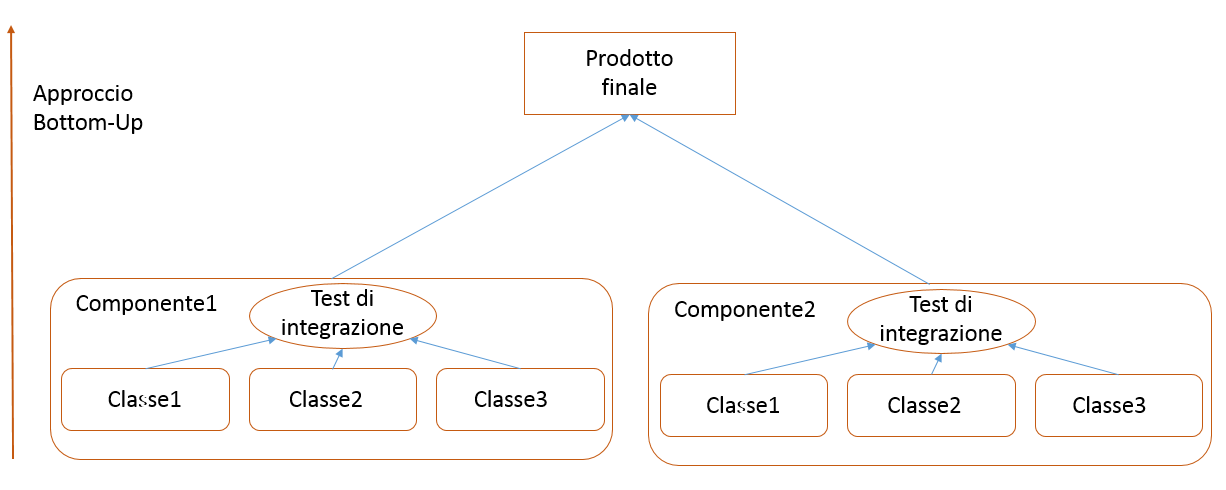
\includegraphics[scale=0.4]{PianoDiQualifica/Pics/bottom-up.png}
			\caption{Modello bottom-up}
		\end{figure}
		\level{3}{Descrizione dei test di integrazione}
			
				\begin{longtabu} spread 1cm [c]{|X[-1,l]|X[-1,l]|X[-1,l]|}
					\hline
					\rowfont{\bf \centering}
					Codice &
					Dettaglio &
					Esito \\
					\hline
					\endhead
					
					TIApplicazione &
                Test di integrazione finale tra tutte le componenti per verificare il corretto comportamento del sistema Applicazione nel suo complesso. &
                Non implementato\\\hline TIApplicazioneModel &
                Viene verificato che il sistema gestisca correttamente la componente Model relativa al design pattern MVP. Più precisamente si verifica che memorizzi correttamente le informazioni relative alla sessione con l'istanza di Norris selezionata nonché i dati riguardanti i chart ottenuti. Si verifica inoltre che la richiesta e l'aggiornamento di un grafico siano gestiti in modo corretto. &
                Non implementato\\\hline TIApplicazioneModelNorrisChart &
                Viene verificato che il modello dei chart memorizzi correttamente le informazioni in base al tipo specifico di grafico ottenuto da un'istanza di Norris. &
                Non implementato\\\hline TIApplicazioneModelService &
                Viene verificato che la richiesta di un grafico a un'istanza di Norris venga gestita in modo corretto; viene inoltre verificata la correttezza della gestione degli aggiornamenti ricevuti dall'istanza di Norris. &
                Non implementato\\\hline TIApplicazionePresenter &
                Viene verificato che il controllo dell'applicazione avvenga nel modo corretto. In particolare si verifica che l'interfacciamento con l'istanza di Norris avvenga in modo corretto (autenticazione e richesta della lista dei grafici); inoltre si verifica che avviene correttamente la gestione degli eventi provenienti dalla view. &
                Non implementato\\\hline TIApplicazioneView &
                Viene verificato che il sistema gestisca correttamente la componente View relativa al design pattern MVP. In particolare, si verifica che sia gestito in modo corretto la rappresentazione dei chart e che siano scatenati gli eventi corretti all'avvenire di determinate user gesture. &
                Non implementato\\\hline TIChuck &
                Test di integrazione finale tra tutte le componenti per verificare il corretto comportamento del sistema Chuck nel suo complesso. &
                Non implementato\\\hline TIChuckDirective &
                Viene verificato che le operazioni fornite allo sviluppatore si comportino in modo appropriato restituendo dati corretti. In particolare si verifica che gli output derivanti dalla gestione delle operazioni (che poi verranno forniti ad altri componenti, View e ViewModel) siano appropriati. &
                Non implementato\\\hline TIChuckModel &
                Viene verificato che il sistema gestisca correttamente la componente Model relativa al design pattern MVC. Più precisamente si verifica che memorizzi correttamente i dati riguardanti i chart ottenuti. Si verifica inoltre che la richiesta e l'aggiornamento di un grafico siano gestiti in modo corretto. &
                Non implementato\\\hline TIChuckModelNorrisChart &
                Viene verificato che il modello dei chart memorizzi correttamente le informazioni in base al tipo specifico di grafico ottenuto da un'istanza di Norris. Viene inoltre verificato che gli aggiornamenti provenienti da Norris vengano eseguiti in modo corretto. &
                Non implementato\\\hline TIChuckModelServices &
                Viene verificato il corretto funzionamento dell'autenticazione a un'istanza di Norris. Viene inoltre verificato che la richiesta di un grafico e la successiva ricezione di dati dall'istanza di Norris siano gestiti in modo corretto. &
                Non implementato\\\hline TIChuckView &
                Viene verificato che un chart venga visualizzato in modo corretto all'interno di una pagina web (anche in seguito ad un'aggiornamento). Si verifica inoltre che siano raccolti e inviati in modo appropriato gli input inerenti il filtraggio dei dati. &
                Non implementato\\\hline TIChuckViewModel &
                Viene verificato che le funzionalità delle librerie grafiche vengano invocate in modo corretto. Inoltre viene verificato che gli input provenienti dalla view (riguardanti il filtraggio dei dati) vengano gestiti in modo corretto. &
                Non implementato\\\hline TINorris &
                Test di integrazione finale tra tutte le componenti per verificare il corretto comportamento del sistema Norris nel suo complesso. &
                Non implementato\\\hline TINorrisDataModel &
                Viene verificato che il comportamento del modello rispetti le aspettative previste, ovvero memorizzi correttamente i dati riguardanti pagine e chart e li restituisca in un secondo momento senza perdite di informazioni o dati scorretti. &
                Non eseguito\\\hline TINorrisDataModelNorrisChart &
                Viene verificato che il modello dei chart memorizzi correttamente le informazioni in base al tipo specifico del chart rappresentato (durante la creazione e l'aggiornamento). &
                Non eseguito\\\hline TINorrisDataModelNorrisPage &
                Viene verificato che il modello memorizzi correttamente le informazioni riguardanti le pagine appartenenti a un'istanza di Norris (grafici in esse contenuti e relative impostazioni). &
                Non eseguito\\\hline TINorrisExternalAPIManager &
                Viene verificato il funzionamento delle API esterne, ovvero si controlla che le API esterne forniscano le funzioni corrette a seconda dei dati rappresentati dal modello. &
                Non implementato\\\hline TINorrisInternalAPIManager &
                Viene verificato il corretto funzionamento delle API interne, ovvero si controlla che le API interne apportino al modello le modifiche corrette a seconda dell'azione richiesta. &
                Non eseguito\\\hline \caption{Test di integrazione}
\end{longtabu}
		\level{3}{Tracciamento test di integrazione - componenti}
			
				\begin{longtabu} spread 1cm [c]{|p{5cm}|p{9cm}|}
					\hline
					\rowfont{\bf \centering}
					Codice &
					Componenti abbinati \\
					\hline
					\endhead
					
					TIApplicazione & \parbox[t]{4cm}{ A001-Applicazione::Model \\ A002-Applicazione::View \\ A003-Applicazione::Presenter }\\
                \hline
                TIApplicazioneModel & \parbox[t]{4cm}{ A001-Applicazione::Model \\ A004-Applicazione::Model::NorrisChart \\ A005-Applicazione::Model::Service }\\
                \hline
                TIApplicazioneModelNorrisChart & \parbox[t]{4cm}{ A004-Applicazione::Model::NorrisChart }\\
                \hline
                TIApplicazioneModelService & \parbox[t]{4cm}{ A005-Applicazione::Model::Service }\\
                \hline
                TIApplicazionePresenter & \parbox[t]{4cm}{ A003-Applicazione::Presenter }\\
                \hline
                TIChuckBarChart & \parbox[t]{4cm}{ C006-Chuck::Model::Services }\\
                \hline
                TIChuckLineChart & \parbox[t]{4cm}{ C005-Chuck::Model::NorrisChart }\\
                \hline
                TIChuckMapChart & \parbox[t]{4cm}{ C002-Chuck::View }\\
                \hline
                TIChuckTable & \parbox[t]{4cm}{ C003-Chuck::ViewModel }\\
                \hline
                TINorris & \parbox[t]{4cm}{ N001-Norris::InternalAPIManager \\ N002-Norris::ExternalAPIManager \\ N003-Norris::DataModel }\\
                \hline
                TINorrisDataModel & \parbox[t]{4cm}{ N004-Norris::DataModel::NorrisChart \\ N005-Norris::DataModel::NorrisPage }\\
                \hline
                TINorrisDataModelNorrisChart & \parbox[t]{4cm}{ N004-Norris::DataModel::NorrisChart }\\
                \hline
                TINorrisDataModelNorrisPage & \parbox[t]{4cm}{ N005-Norris::DataModel::NorrisPage }\\
                \hline
                TINorrisExternalAPIManager & \parbox[t]{4cm}{ N002-Norris::ExternalAPIManager }\\
                \hline
                TINorrisInternalAPIManager & \parbox[t]{4cm}{ N001-Norris::InternalAPIManager }\\
                \hline
                                \caption{Tracciamento test-componenti}
				\end{longtabu}
				
	\level{2}{Test di unità}
		Di seguito vengono riportati i test di unità, ovvero quei test che servono per verificare il corretto funzionamento delle singole unità, ovvero le classi. Per una descrizione completa della sintassi utilizzata nella descrizione di tali test si consulti il documento \insdoc{Norme di Progetto v6.00}.
		\level{3}{Descrizione dei test di unità}
			
				\begin{longtabu} spread 1cm [c]{|X[-1,l]|X[-1,l]|X[-1,l]|}
					\hline
					\rowfont{\bf \centering}
					Codice &
					Dettaglio &
					Esito \\
					\hline
					\endhead
					
					TUA-BarChartActivity01 &
                Viene testato che tramite la classe BarChartActivity sia possibile visualizzare grafici di tipo BarChart e modificarne le impostazioni di visualizzazione. &
                Superato\\\hline TUA-BarChartDataImpl01 &
                Viene testato che un oggetto BarChartDataImpl memorizzi correttamente i valori del chart e permetta di ottenere e modificare tali dati &
                Superato\\\hline TUA-BarChartElementInPlaceUpdate &
                Viene testato che un oggetto BarChartElementUpdate memorizzi correttamente il valore dell'aggiornamento in place per un elemento di un BarChart e che permetta di ottenere le sue proprietà &
                Superato\\\hline TUA-BarChartImpl01 &
                Viene testato che sia correttamente registrata la sua classe factory &
                Superato\\\hline TUA-BarChartInPlaceUpdate01 &
                Viene testato che un oggetto BarChartInPlaceUpdate memorizzi correttamente un pacchetto di aggiornamento In Place per un BarChart e che permetta di ottenere le sue proprietà &
                Superato\\\hline TUA-BarChartInPlaceUpdater01 &
                Viene testato che il metodo di aggiornamento in place di un grafico BarChart funzioni correttamente &
                Superato\\\hline TUA-BarChartPresenterImpl01 &
                Viene testato che i dati contenuti nel modello di BarChart siano correttamente inviati alla View per essere rappresentati e che ne vengano inizializzate le corrette impostazioni. &
                Superato\\\hline TUA-BarChartPresenterImpl02 &
                Viene testato che: alla creazione venga correttamente richiesto il BarChart associato al presenter; all'ottenimento dei vari dati (dati e impostazioni) vengano trasformati e creato il modello; vengano attivati gli aggiornamenti di tale chart. &
                Superato\\\hline TUA-BarChartSettingsImpl01 &
                Viene testato che un oggetto BarChartSettingsImpl memorizzi correttamente le impostazioni del chart e permetta di ottenere le sue proprietà &
                Superato\\\hline TUA-BaseActivity01 &
                Viene testato che sia possibile creare una activity &
                Superato\\\hline TUA-ChartActivity01 &
                Viene verificato che sia possibile creare una activity con un grafico &
                Superato\\\hline TUA-ChartImpl01 &
                Viene testato che sia possibile implementare un grafico generico a cui passare dei dati e inizializzare delle impostazioni &
                Superato\\\hline TUA-ChartPresenterImpl01 &
                Viene testato che i dati contenuti nel modello di un grafico siano correttamente inviati alla View per essere rappresentati &
                Superato\\\hline TUA-ChartReceiverImpl01 &
                Viene testato che sia possibile ricevere correttamente eventi di tipo update o chart dall'istanza di Norris attraverso il canale socket &
                Superato\\\hline TUA-ChartReceiverImpl02 &
                Viene testato che sia possibile inviare correttamente richieste di tipo update o chart all'istanza di Norris attraverso il canale socket &
                Superato\\\hline TUA-HttpRequesterWithCookie01 &
                Viene testato che il metodo di login consenta l'accesso ad una istanza di Norris solo previo inserimento delle credenziali stabilite e ne vengano salvati sul modello le informazioni sullo stato della sessione. &
                Superato\\\hline TUA-HttpRequesterWithCookie02 &
                Viene testato che il metodo di logout consenta di disconnettersi da una istanza di Norris e ne vengano salvati sul modello le informazioni sullo stato della sessione. &
                Superato\\\hline TUA-HttpRequesterWithCookie03 &
                Viene testato che sia possibile ottenere la lista di grafici presenti in una istanza di Norris tramite una richiesta http e ne vengano salvati sul modello le informazioni sullo stato della sessione. &
                Superato\\\hline TUA-HttpRequesterWithCookie04 &
                Viene testato che sia possibile verificare l'avvenuta autenticazione presso una istanza protetta di Norris e ne vengano salvati sul modello le informazioni sullo stato della sessione. &
                Superato\\\hline TUA-JSONParser01 &
                Viene testato che i vari oggetti JSON per dati, impostazioni e aggiornamenti vengano correttamente convertiti nel formato corretto. &
                Superato\\\hline TUA-LineChartActivity01 &
                Viene testato che tramite la classe LineChartActivity sia possibile visualizzare grafici di tipo LineChart e modificarne le impostazioni di visualizzazione. &
                Superato\\\hline TUA-LineChartDataImpl01 &
                Viene testato che un oggetto LineChartDataImpl memorizzi correttamente i valori del chart e permetta di ottenere e modificare tali dati &
                Superato\\\hline TUA-LineChartElementInPlaceUpdate01 &
                Viene testato che un oggetto LineChartElementInPlaceUpdate memorizzi correttamente il valore dell'aggiornamento In Place per un elemento di un LineChart e che permetta di ottenere le sue proprietà &
                Superato\\\hline TUA-LineChartElementStreamUpdate01 &
                Viene testato che un oggetto LineChartElementStreamUpdate memorizzi correttamente il valore dell'aggiornamento Stream per un elemento di un LineChart e che permetta di ottenere le sue proprietà &
                Superato\\\hline TUA-LineChartImpl01 &
                Viene testato che sia correttamente registrata la sua classe factory &
                Superato\\\hline TUA-LineChartInPlaceUpdate01 &
                Viene testato che un oggetto LineChartUpdate memorizzi correttamente un pacchetto di aggiornamento In Place per un LineChart e che permetta di ottenere le sue proprietà. &
                Superato\\\hline TUA-LineChartInPlaceUpdater01 &
                Viene testato che il metodo di aggiornamento in place di un grafico LineChart funzioni correttamente &
                Superato\\\hline TUA-LineChartInStreamUpdater01 &
                Viene testato che il metodo di aggiornamento in stream in un grafico LineChart funzioni correttamente &
                Superato\\\hline TUA-LineChartPresenterImpl01 &
                Viene testato che i dati contenuti nel modello di LineChart siano correttamente inviati alla View per essere rappresentati e che ne vengano inizializzate le corrette impostazioni. &
                Superato\\\hline TUA-LineChartPresenterImpl02 &
                Viene testato che: alla creazione venga correttamente richiesto il LineChart associato al presenter; all'ottenimento dei vari dati (dati e impostazioni) vengano trasformati e creato il modello; vengano attivati gli aggiornamenti di tale chart. &
                Superato\\\hline TUA-LineChartSettingsImpl01 &
                Viene testato che un oggetto LineChartSettingsImpl memorizzi correttamente le impostazioni del chart e permetta di ottenere le sue proprietà &
                Superato\\\hline TUA-LineChartStreamUpdate01 &
                Viene testato che un oggetto LineChartStreamUpdate memorizzi correttamente un pacchetto di aggiornamento Stream per un LineChart e che permetta di ottenere le sue proprietà &
                Superato\\\hline TUA-ListActivity01 &
                Viene testato che: sia possibile visualizzare la lista dei grafici contenuti in una istanza di Norris e delle informazioni previste per ognuno di essi; sia possibile richiedere il logout. &
                Superato\\\hline TUA-ListPresenterImpl01 &
                Viene testato che la lista di grafici contenuti nel modello di una sessione siano correttamente utilizzati per accedere alla View di una lista di grafici di una istanza di Norris &
                Superato\\\hline TUA-LoginActivity01 &
                Viene testato che sia possibile visualizzare la schermata per l'inserimento delle credenziali con cui accedere ad una istanza protetta di Norris &
                Superato\\\hline TUA-LoginPresenterImpl01 &
                Viene testato che i dati contenuti nel modello di una sessione siano correttamente utilizzati per accedere alla View di per interagire con una istanza di Norris &
                Superato\\\hline TUA-MapChartActivity01 &
                Viene testato che tramite la classe MapChartActivity sia possibile visualizzare grafici di tipo MapChart e modificarne le impostazioni di visualizzazione. &
                Superato\\\hline TUA-MapChartDataImpl01 &
                Viene testato che un oggetto MapChartDataImpl memorizzi correttamente i valori del chart e permetta di ottenere e modificare tali dati &
                Superato\\\hline TUA-MapChartDeleteUpdate01 &
                Viene testato che un oggetto MapChartDeleteUpdate effettui correttamente la cancellazione di un pacchetto per un MapChart e che permetta di ottenere le sue proprietà. &
                Superato\\\hline TUA-MapChartElementInPlaceUpdate01 &
                Viene testato che un oggetto MapChartElementInPlaceUpdate memorizzi correttamente il valore dell'aggiornamento  per un elemento di un MapChart e che permetta di ottenere le sue proprietà. &
                Superato\\\hline TUA-MapChartImpl01 &
                Viene testato che sia correttamente registrata la sua classe factory &
                Superato\\\hline TUA-MapChartInMovieUpdater01 &
                Viene testato che il metodo di aggiornamento in movie di un grafico MapChart funzioni correttamente &
                Superato\\\hline TUA-MapChartInPlaceUpdate01 &
                Viene testato che un oggetto MapChartInPlaceUpdate memorizzi correttamente un pacchetto di aggiornamento In Place per un MapChart e che permetta di ottenere le sue proprietà &
                Superato\\\hline TUA-MapChartInPlaceUpdater01 &
                Viene testato che il metodo di aggiornamento in place di un grafico MapChart funzioni correttamente &
                Superato\\\hline TUA-MapChartMovieUpdate01 &
                Viene testato che un oggetto MapChartMovieUpdate memorizzi correttamente un pacchetto di aggiornamento Movie per una MapChart e che permetta di ottenere le sue proprietà &
                Superato\\\hline TUA-MapChartPresenterImpl01 &
                Viene testato che i dati contenuti nel modello di MapChart siano correttamente inviati alla View per essere rappresentati e che ne vengano inizializzate le corrette impostazioni. &
                Superato\\\hline TUA-MapChartPresenterImpl02 &
                Viene testato che: alla creazione venga correttamente richiesto il MapChart associato al presenter; all'ottenimento dei vari dati (dati e impostazioni) vengano trasformati e creato il modello; vengano attivati gli aggiornamenti di tale chart. &
                Superato\\\hline TUA-MapChartSettingsImpl01 &
                Viene testato che un oggetto MapChartSettingsImpl memorizzi correttamente le impostazioni del chart e permetta di ottenere le sue proprietà. &
                Superato\\\hline TUA-MapChartStreamUpdate01 &
                Viene testato che un oggetto MapChartStreamUpdate memorizzi correttamente un pacchetto di aggiornamento Stream per un MapChart e che permetta di ottenere le sue proprietà. &
                Superato\\\hline TUA-MapPoint01 &
                Viene testato che un oggetto MapPoint memorizzi correttamente i valori di un punto e permetta di ottenerli e modificarli &
                Superato\\\hline TUA-MapSet01 &
                Viene testato che un oggetto MapSet memorizzi correttamente i valori di una serie di dati e permetta di ottenerli e modificarli &
                Superato\\\hline TUA-NorrisSessionInfoImpl01 &
                Viene testato che i dati relativi alle sessioni siano salvati correttamente attraverso i cookie &
                Superato\\\hline TUA-PresenterImpl01 &
                Viene testato che il chart venga creato correttamente nel modello e che ne siano visualizzi valori e impostazioni nella relativa view &
                Superato\\\hline TUA-TableActivity01 &
                Viene testato che tramite la classe TableActivity sia possibile visualizzare grafici di tipo Table e modificarne le impostazioni di visualizzazione. &
                Superato\\\hline TUA-TableCell01 &
                Viene testato che un oggetto TableCell memorizzi correttamente i valori di una cella della tabella e permetta di ottenerli e modificarli &
                Superato\\\hline TUA-TableCellInPlaceUpdate01 &
                Viene testato che un oggetto TableCellInPlaceUpdate memorizzi correttamente il valore dell'aggiornamento In Place per una cella di una Table e che permetta di ottenere le sue proprietà &
                Superato\\\hline TUA-TableDataImpl01 &
                Viene testato che un oggetto TableDataImpl memorizzi correttamente i valori del chart e permetta di ottenere e modificare tali dati &
                Superato\\\hline TUA-TableImpl01 &
                Viene testato che sia correttamente registrata la sua classe factory &
                Superato\\\hline TUA-TableInPlaceUpdate01 &
                Viene testato che un oggetto tableInPlaceUpdate memorizzi correttamente un pacchetto di aggiornamento In Place per una Table e che permetta di ottenere le sue proprietà. &
                Superato\\\hline TUA-TableInPlaceUpdater01 &
                Viene testato che il metodo di aggiornamento in place di un grafico Table funzioni correttamente &
                Superato\\\hline TUA-TableInStreamUpdater01 &
                Viene testato che il metodo di aggiornamento in stream in un grafico Table funzioni correttamente &
                Superato\\\hline TUA-TablePresenterImpl01 &
                Viene testato che i dati contenuti nel modello di Table siano correttamente inviati alla View per essere rappresentati e che ne vengano inizializzate le corrette impostazioni. &
                Superato\\\hline TUA-TablePresenterImpl02 &
                Viene testato che alla creazione venga correttamente richiesta la Table associata al presenter, all'ottenimento dei vari dati (dati e impostazioni) vengano trasformati e creato il modello, vengano attivati gli aggiornamenti di tale chart. &
                Superato\\\hline TUA-TableRow01 &
                Viene testato che un oggetto TableRow memorizzi correttamente i valori di una riga di dati e permetta di ottenerli e modificarli &
                Superato\\\hline TUA-TableSettingsImpl01 &
                Viene testato che un oggetto TableSettingsImpl memorizzi correttamente le impostazioni del chart e permetta di ottenere le sue proprietà &
                Superato\\\hline TUA-TableStreamUpdate01 &
                Viene testato che un oggetto TableStreamUpdate memorizzi correttamente un pacchetto di aggiornamento Stream per una Table e che permetta di ottenere le sue proprietà &
                Superato\\\hline TUC-BarChartImpl01 &
                Viene testato che sia correttamente registrata la sua classe factory &
                Superato\\\hline TUC-BarChartInPlaceUpdater01 &
                Viene testato che il metodo di aggiornamento in place di un grafico BarChart funzioni correttamente &
                Superato\\\hline TUC-BarChartView01 &
                Viene testato che risulti graficamente visibile il cambiamento di dati e impostazioni di un BarChart &
                Superato\\\hline TUC-BarChartViewModel01 &
                Viene testato che la libreria grafica Chart.js fornisca una corretta rappresentazione grafica di un BarChart &
                Superato\\\hline TUC-ChartImpl01 &
                Viene testato che sia possibile implementare un grafico generico a cui passare dei dati e inizializzare delle impostazioni &
                Superato\\\hline TUC-ChartRequester01 &
                Viene testato che sia possibile ottenere e mantenere aggiornati i grafici da una istanza di Norris &
                Superato\\\hline TUC-ChartView01 &
                Viene testato che risulti graficamente visibile il cambiamento di dati e impostazioni di un grafico &
                Superato\\\hline TUC-ChuckBarChart01 &
                Viene testato che sia possibile inserire un BarChart all'interno di una pagina web &
                Superato\\\hline TUC-ChuckLineChart01 &
                Viene testato che sia possibile inserire un LineChart all'interno di una pagina web &
                Superato\\\hline TUC-ChuckMapChart01 &
                Viene testato che sia possibile inserire un LMapChart all'interno di una pagina web &
                Superato\\\hline TUC-ChuckTable01 &
                Viene testato che sia possibile inserire una Table all'interno di una pagina web &
                Superato\\\hline TUC-LineChartImpl01 &
                Viene testato che sia correttamente registrata la sua classe factory &
                Superato\\\hline TUC-LineChartInPlaceUpdater01 &
                Viene testato che il metodo di aggiornamento in place di un grafico LineChart funzioni correttamente &
                Superato\\\hline TUC-LineChartStreamUpdater01 &
                Viene testato che il metodo di aggiornamento in stream di un grafico LineChart funzioni correttamente &
                Superato\\\hline TUC-LineChartView01 &
                Viene testato che risulti graficamente visibile il cambiamento di dati e impostazioni dei un LineChart &
                Superato\\\hline TUC-LineChartViewModel01 &
                Viene testato che la libreria grafica Chart.js fornisca una corretta rappresentazione grafica di un LineChart &
                Superato\\\hline TUC-MapChartImpl01 &
                Viene testato che sia correttamente registrata la sua classe factory &
                Superato\\\hline TUC-MapChartInPlaceUpdater01 &
                Viene testato che il metodo di aggiornamento in place di un grafico MapChart funzioni correttamente &
                Superato\\\hline TUC-MapChartMovieUpdater01 &
                Viene testato che il metodo di aggiornamento in stream di un grafico MapChart funzioni correttamente &
                Superato\\\hline TUC-MapChartView01 &
                Viene testato che risulti graficamente visibile il cambiamento di dati e impostazioni di un MapChart &
                Superato\\\hline TUC-MapChartViewModel01 &
                Viene testato che la libreria grafica OpenStreetMap fornisca una corretta rappresentazione grafica di un MapChart &
                Superato\\\hline TUC-TableImpl01 &
                Viene testato che sia correttamente registrata la sua classe factory &
                Superato\\\hline TUC-TableInPlaceUpdater01 &
                Viene testato che il metodo di aggiornamento in place di una Table funzioni correttamente &
                Superato\\\hline TUC-TableStreamUpdater01 &
                Viene testato che il metodo di aggiornamento in stream di una Table funzioni correttamente &
                Superato\\\hline TUC-TableView01 &
                Viene testato che risulti graficamente visibile il cambiamento di dati e impostazioni di una Table &
                Superato\\\hline TUC-TableViewModel01 &
                Viene testato che la libreria grafica Dynatable fornisca una corretta rappresentazione grafica di una Table &
                Superato\\\hline TUN-AuthenticationEndpoint01 &
                Viene testato che sia possibile autenticarsi presso un'istanza di Norris fornendo le credenziali corrette &
                Superato\\\hline TUN-AuthenticationEndpoint02 &
                Viene testato che sia possibile scollegarsi da una istanza protetta di Norris a cui ci si è precedentemente loggati &
                Superato\\\hline TUN-AuthenticationEndpoint03 &
                Viene testato il corretto funzionamento del metodo che controlla se è stato effettuato il login ad una istanza protetta di Norris &
                Superato\\\hline TUN-BarChartImpl01 &
                Viene testato che sia correttamente registrata la sua classe factory &
                Superato\\\hline TUN-BarChartInPlaceUpdater01 &
                Viene testato che sia possibile aggiornare il grafico BarChart attraverso il metodo in place &
                Superato\\\hline TUN-ChartBridge01 &
                Viene testato che le richieste di modifica delle impostazioni e di aggiornamento dei grafici siano correttamente inoltrate al modello dei dati &
                Superato\\\hline TUN-ChartEndpoint01 &
                Viene testato che le richieste dei grafici da parte del client e l'invio dei loro aggiornamenti siano gestiti correttamente &
                Superato\\\hline TUN-ChartImpl01 &
                Viene testato che sia possibile creare istanze di grafici a cui passare dei dati, inizializzare le impostazioni e selezionare il tipo di aggiornamento &
                Superato\\\hline TUN-ChartRef01 &
                Viene testato che sia possibile ottenere l'ID, il tipo, i dati e le impostazioni di un grafico da parte di un client &
                Superato\\\hline TUN-ExternalAPIConstructor01 &
                Viene testato che, dopo la creazione di una sola istanza di ExternalAPIController, essa venga associata correttamente ad ogni Endpoint &
                Superato\\\hline TUN-ExternalAPIController01 &
                Viene testato che, una volta registrati gli endpoint, sia possibile restituire loro uno o più grafici presenti in una istanza di Norris &
                Superato\\\hline TUN-ExternalAPIController02 &
                Viene testato che, una volta registrati gli endpoint, sia possibile autenticarsi ad una istanza protetta di Norris &
                Superato\\\hline TUN-ExternalAPIController03 &
                Viene testato che, una volta registrati gli endpoint, sia possibile scollegarsi da una istanza protetta di Norris a cui ci si era precedentemente loggati &
                Superato\\\hline TUN-ExternalAPIController04 &
                Viene testato che, una volta registrati gli endpoint, sia possibile verificare l'avvenuta autenticazione  ad una istanza protetta di Norris &
                Superato\\\hline TUN-LineChartImpl01 &
                Viene testato che sia correttamente registrata la sua classe factory &
                Superato\\\hline TUN-LineChartInPlaceUpdater01 &
                Viene testato che sia possibile aggiornare il grafico LineChart attraverso il metodo in place &
                Superato\\\hline TUN-LineChartInStreamUpdater01 &
                Viene testato che sia possibile aggiornare il grafico LineChart attraverso il metodo in stream &
                Superato\\\hline TUN-ListEndpoint01 &
                Viene testato che, al momento della richiesta della lista di grafici, il client sia correttamente autenticato ad una istanza di Norris per poter ricevere la lista &
                Superato\\\hline TUN-MapChartImpl01 &
                Viene testato che sia correttamente registrata la sua classe factory &
                Superato\\\hline TUN-MapChartInPlaceUpdater01 &
                Viene testato che sia possibile aggiornare il grafico MapChart attraverso il metodo in place &
                Superato\\\hline TUN-MapChartMovieUpdater01 &
                Viene testato che sia possibile aggiornare il grafico MapChart attraverso il metodo movie &
                Superato\\\hline TUN-NorrisBridge01 &
                Viene testato che le richieste di modifica delle impostazioni siano correttamente inviate a un'istanza di Norris &
                Superato\\\hline TUN-NorrisBridge02 &
                Viene testato che le funzioni di autenticazione siano correttamente inviate a un'istanza di Norris &
                Superato\\\hline TUN-NorrisBridge03 &
                Viene testato che le richieste di aggiunta di grafici e pagine siano correttamente inviate ad una istanza di Norris &
                Superato\\\hline TUN-NorrisImpl &
                Viene testato che sia possibile creare una istanza di Norris in cui inizializzare le impostazioni, creare e gestire pagine e grafici &
                Superato\\\hline TUN-PageBridge01 &
                Viene testato che le richieste di modifica di impostazioni di una pagina siano correttamente inviate ad una istanza di pagina &
                Superato\\\hline TUN-PageBridge02 &
                Viene testato che le richieste di aggiunta di grafici siano correttamente inviate ad una istanza di pagina &
                Superato\\\hline TUN-TableImpl01 &
                Viene testato che sia correttamente registrata la sua classe factory &
                Superato\\\hline TUN-TableInPlaceUpdater01 &
                Viene testato che sia possibile aggiornare una Table attraverso il metodo in place &
                Superato\\\hline TUN-TableStreamUpdater01 &
                Viene testato che sia possibile aggiornare una Table attraverso il metodo in stream &
                Superato\\\hline \caption{Test di unità}
\end{longtabu}
		\level{3}{Tracciamento test di unità - classi/metodi}
			
				\begin{longtabu} spread 1cm [c]{|p{6cm}|p{8cm}|}
					\hline
					\rowfont{\bf \centering}
					Codice &
					Classe.metodo \\
					\hline
					\endhead
					
					TUA-BarChartActivity01 & \parbox[t]{4cm}{ Applicazione::View::BarChartActivity.setAxis \\ Applicazione::View::BarChartActivity.renderChart \\ Applicazione::View::BarChartActivity.setAxisName \\ Applicazione::View::BarChartActivity.setLegendPosition \\ Applicazione::View::BarChartActivity.setOrientation \\ Applicazione::View::BarChartActivity.setSeries \\ Applicazione::View::BarChartActivity.setTitle \\ Applicazione::View::BarChartActivity.showGrid }\\
                \hline
                TUA-BarChartDataImpl01 & \parbox[t]{4cm}{ Applicazione::Model::NorrisChart::BarChartDataImpl.getData \\ Applicazione::Model::NorrisChart::BarChartDataImpl.setData }\\
                \hline
                TUA-BarChartElementInPlaceUpdate & \parbox[t]{4cm}{ Applicazione::Model::NorrisChart::BarChartElementInPlaceUpdate.getData \\ Applicazione::Model::NorrisChart::BarChartElementInPlaceUpdate.getX \\ Applicazione::Model::NorrisChart::BarChartElementInPlaceUpdate.getY }\\
                \hline
                TUA-BarChartImpl01 & \parbox[t]{4cm}{ Chuck::Model::NorrisChart::BarChartImpl }\\
                \hline
                TUA-BarChartInPlaceUpdate01 & \parbox[t]{4cm}{ Applicazione::Model::NorrisChart::BarChartInPlaceUpdate.getData }\\
                \hline
                TUA-BarChartInPlaceUpdater01 & \parbox[t]{4cm}{ Applicazione::Model::NorrisChart::BarChartInPlaceUpdater.update }\\
                \hline
                TUA-BarChartPresenterImpl01 & \parbox[t]{4cm}{ Applicazione::Presenter::BarChartPresenterImpl.update \\ Applicazione::Presenter::BarChartPresenterImpl.applySettings }\\
                \hline
                TUA-BarChartPresenterImpl02 & \parbox[t]{4cm}{ Applicazione::Presenter::BarChartPresenterImpl }\\
                \hline
                TUA-BarChartSettingsImpl01 & \parbox[t]{4cm}{ Applicazione::Model::NorrisChart::BarChartSettingsImpl.getGridVisibility \\ Applicazione::Model::NorrisChart::BarChartSettingsImpl.getLegendPosition \\ Applicazione::Model::NorrisChart::BarChartSettingsImpl.getOrientation \\ Applicazione::Model::NorrisChart::BarChartSettingsImpl.getXAxisName \\ Applicazione::Model::NorrisChart::BarChartSettingsImpl.getYAxisName }\\
                \hline
                TUA-BaseActivity01 & \parbox[t]{4cm}{ Applicazione::View::BaseActivity }\\
                \hline
                TUA-ChartActivity01 & \parbox[t]{4cm}{ Applicazione::View::ChartActivity.renderChart \\ Applicazione::View::ChartActivity.setTitle \\ Applicazione::View::ChartActivity.getChartId }\\
                \hline
                TUA-ChartImpl01 & \parbox[t]{4cm}{ Applicazione::Model::NorrisChart::ChartImpl.create \\ Applicazione::Model::NorrisChart::ChartImpl.getData \\ Applicazione::Model::NorrisChart::ChartImpl.getId \\ Applicazione::Model::NorrisChart::ChartImpl.getSettings \\ Applicazione::Model::NorrisChart::ChartImpl.getType \\ Applicazione::Model::NorrisChart::ChartImpl.setData \\ Applicazione::Model::NorrisChart::ChartImpl.setSettings \\ Applicazione::Model::NorrisChart::ChartImpl.update }\\
                \hline
                TUA-ChartPresenterImpl01 & \parbox[t]{4cm}{ Applicazione::Presenter::ChartPresenterImpl.update }\\
                \hline
                TUA-ChartReceiverImpl01 & \parbox[t]{4cm}{ Applicazione::Model::Service::ChartReceiverImpl.startUpdateEvent \\ Applicazione::Model::Service::ChartReceiverImpl.stopUpdateEvent }\\
                \hline
                TUA-ChartReceiverImpl02 & \parbox[t]{4cm}{ Applicazione::Model::Service::ChartReceiverImpl.getChart }\\
                \hline
                TUA-HttpRequesterWithCookie01 & \parbox[t]{4cm}{ Applicazione::Presenter::HttpRequesterWithCookie.login }\\
                \hline
                TUA-HttpRequesterWithCookie02 & \parbox[t]{4cm}{ Applicazione::Presenter::HttpRequesterWithCookie.logout }\\
                \hline
                TUA-HttpRequesterWithCookie03 & \parbox[t]{4cm}{ Applicazione::Presenter::HttpRequesterWithCookie.getList }\\
                \hline
                TUA-HttpRequesterWithCookie04 & \parbox[t]{4cm}{ Applicazione::Presenter::HttpRequesterWithCookie.keepAlive }\\
                \hline
                TUA-JSONParser01 & \parbox[t]{4cm}{ Applicazione::Presenter::JSONParser.parseUpdate \\ Applicazione::Presenter::JSONParser.parseChart \\ Applicazione::Presenter::JSONParser.parseSettings }\\
                \hline
                TUA-LineChartActivity01 & \parbox[t]{4cm}{ Applicazione::View::LineChartActivity.renderChart \\ Applicazione::View::LineChartActivity.setAxisName \\ Applicazione::View::LineChartActivity.setDottedLines \\ Applicazione::View::LineChartActivity.showGrid \\ Applicazione::View::LineChartActivity.setLegendPosition \\ Applicazione::View::LineChartActivity.setSeriesColor }\\
                \hline
                TUA-LineChartDataImpl01 & \parbox[t]{4cm}{ Applicazione::Model::NorrisChart::LineChartDataImpl.getData \\ Applicazione::Model::NorrisChart::LineChartDataImpl.setData }\\
                \hline
                TUA-LineChartElementInPlaceUpdate01 & \parbox[t]{4cm}{ Applicazione::Model::NorrisChart::LineChartElementInPlaceUpdater.getData \\ Applicazione::Model::NorrisChart::LineChartElementInPlaceUpdater.getX \\ Applicazione::Model::NorrisChart::LineChartElementInPlaceUpdater.getY }\\
                \hline
                TUA-LineChartElementStreamUpdate01 & \parbox[t]{4cm}{ Applicazione::Model::NorrisChart::LineChartElementStreamUpdate.getData \\ Applicazione::Model::NorrisChart::LineChartElementStreamUpdate.getLabel }\\
                \hline
                TUA-LineChartImpl01 & \parbox[t]{4cm}{ Applicazione::Model::NorrisChart::LineChartImpl }\\
                \hline
                TUA-LineChartInPlaceUpdate01 & \parbox[t]{4cm}{ Applicazione::Model::NorrisChart::LineChartInPlaceUpdate.getData }\\
                \hline
                TUA-LineChartInPlaceUpdater01 & \parbox[t]{4cm}{ Applicazione::Model::NorrisChart::LineChartInPlaceUpdater.update }\\
                \hline
                TUA-LineChartInStreamUpdater01 & \parbox[t]{4cm}{ Applicazione::Model::NorrisChart::LineChartStreamUpdater.update }\\
                \hline
                TUA-LineChartPresenterImpl01 & \parbox[t]{4cm}{ Applicazione::Presenter::LineChartPresenterImpl.update \\ Applicazione::Presenter::LineChartPresenterImpl.applySettings }\\
                \hline
                TUA-LineChartPresenterImpl02 & \parbox[t]{4cm}{ Applicazione::Presenter::LineChartPresenterImpl }\\
                \hline
                TUA-LineChartSettingsImpl01 & \parbox[t]{4cm}{ Applicazione::Model::NorrisChart::LineChartSettingsImpl.getGridVisibility \\ Applicazione::Model::NorrisChart::LineChartSettingsImpl.getLegendPosition \\ Applicazione::Model::NorrisChart::LineChartSettingsImpl.getXAxisName \\ Applicazione::Model::NorrisChart::LineChartSettingsImpl.getYAxisName }\\
                \hline
                TUA-LineChartStreamUpdate01 & \parbox[t]{4cm}{ Applicazione::Model::NorrisChart::LineChartStreamUpdate.getData }\\
                \hline
                TUA-ListActivity01 & \parbox[t]{4cm}{ Applicazione::View::ListActivity.navigate \\ Applicazione::View::ListActivity.onItemClick \\ Applicazione::View::ListActivity.onLogoutClick \\ Applicazione::View::ListActivity.renderList \\ Applicazione::View::ListActivity.showChartDetailView }\\
                \hline
                TUA-ListPresenterImpl01 & \parbox[t]{4cm}{ Applicazione::Presenter::ListPresenterImpl.onResume \\ Applicazione::Presenter::ListPresenterImpl.onItemClicked \\ Applicazione::Presenter::ListPresenterImpl.onLogoutClick }\\
                \hline
                TUA-LoginActivity01 & \parbox[t]{4cm}{ Applicazione::View::LoginActivity.showAuthenticationError \\ Applicazione::View::LoginActivity.showListView \\ Applicazione::View::LoginActivity.showProgress \\ Applicazione::View::LoginActivity.onLoginClick }\\
                \hline
                TUA-LoginPresenterImpl01 & \parbox[t]{4cm}{ Applicazione::Presenter::LoginPresenterImpl.onLoginClick }\\
                \hline
                TUA-MapChartActivity01 & \parbox[t]{4cm}{ Applicazione::View::MapChartActivity.render \\ Applicazione::View::MapChartActivity.setCameraCoordinate \\ Applicazione::View::MapChartActivity.setCameraZoom \\ Applicazione::View::MapChartActivity.setMarkerShape \\ Applicazione::View::MapChartActivity.setSeriesColor }\\
                \hline
                TUA-MapChartDataImpl01 & \parbox[t]{4cm}{ Applicazione::Model::NorrisChart::MapChartDataImpl.getData \\ Applicazione::Model::NorrisChart::MapChartDataImpl.setData }\\
                \hline
                TUA-MapChartDeleteUpdate01 & \parbox[t]{4cm}{ Applicazione::Model::NorrisChart::MapChartDeleteUpdate.getData }\\
                \hline
                TUA-MapChartElementInPlaceUpdate01 & \parbox[t]{4cm}{ Applicazione::Model::NorrisChart::MapChartElementInPlaceUpdate.getData \\ Applicazione::Model::NorrisChart::MapChartElementInPlaceUpdate.getId \\ Applicazione::Model::NorrisChart::MapChartElementInPlaceUpdate.getX \\ Applicazione::Model::NorrisChart::MapChartElementInPlaceUpdate.getY }\\
                \hline
                TUA-MapChartImpl01 & \parbox[t]{4cm}{ Applicazione::Model::NorrisChart::MapChartImpl }\\
                \hline
                TUA-MapChartInMovieUpdater01 & \parbox[t]{4cm}{ Applicazione::Model::NorrisChart::MapChartMovieUpdater.update }\\
                \hline
                TUA-MapChartInPlaceUpdate01 & \parbox[t]{4cm}{ Applicazione::Model::NorrisChart::MapChartInPlaceUpdate.getData }\\
                \hline
                TUA-MapChartInPlaceUpdater01 & \parbox[t]{4cm}{ Applicazione::Model::NorrisChart::MapChartInPlaceUpdater.update }\\
                \hline
                TUA-MapChartMovieUpdate01 & \parbox[t]{4cm}{ Applicazione::Model::NorrisChart::MapChartMovieUpdate.getDeleteData \\ Applicazione::Model::NorrisChart::MapChartMovieUpdate.getInPlaceData \\ Applicazione::Model::NorrisChart::MapChartMovieUpdate.getStreamData }\\
                \hline
                TUA-MapChartPresenterImpl01 & \parbox[t]{4cm}{ Applicazione::Presenter::MapChartPresenterImpl.update \\ Applicazione::Presenter::MapChartPresenterImpl.applySettings }\\
                \hline
                TUA-MapChartPresenterImpl02 & \parbox[t]{4cm}{ }\\
                \hline
                TUA-MapChartSettingsImpl01 & \parbox[t]{4cm}{ Applicazione::Model::NorrisChart::MapChartSettingsImpl.getCameraZoomHeight \\ Applicazione::Model::NorrisChart::MapChartSettingsImpl.getMarkerType \\ Applicazione::Model::NorrisChart::MapChartSettingsImpl.getXCameraCoordinate \\ Applicazione::Model::NorrisChart::MapChartSettingsImpl.getYCameraCoordinate }\\
                \hline
                TUA-MapChartStreamUpdate01 & \parbox[t]{4cm}{ Applicazione::Model::NorrisChart::MapChartStreamUpdate.getData }\\
                \hline
                TUA-MapPoint01 & \parbox[t]{4cm}{ Applicazione::Model::NorrisChart::MapPoint.getId \\ Applicazione::Model::NorrisChart::MapPoint.getLatitude \\ Applicazione::Model::NorrisChart::MapPoint.getLongitude \\ Applicazione::Model::NorrisChart::MapPoint.setLatitude \\ Applicazione::Model::NorrisChart::MapPoint.setLongitude }\\
                \hline
                TUA-MapSet01 & \parbox[t]{4cm}{ Applicazione::Model::NorrisChart::MapSet.getData \\ Applicazione::Model::NorrisChart::MapSet.setData }\\
                \hline
                TUA-NorrisSessionInfoImpl01 & \parbox[t]{4cm}{ Applicazione::Model::NorrisSessionInfoImpl.getAddress \\ Applicazione::Model::NorrisSessionInfoImpl.setAddress \\ Applicazione::Model::NorrisSessionInfoImpl.login \\ Applicazione::Model::NorrisSessionInfoImpl.logout \\ Applicazione::Model::NorrisSessionInfoImpl.isLogged \\ Applicazione::Model::NorrisSessionInfoImpl.getAuthCookie }\\
                \hline
                TUA-PresenterImpl01 & \parbox[t]{4cm}{ Applicazione::Presenter::PresenterImpl.registerFactory \\ Applicazione::Presenter::PresenterImpl.create }\\
                \hline
                TUA-TableActivity01 & \parbox[t]{4cm}{ Applicazione::View::TableActivity.renderChart \\ Applicazione::View::TableActivity.setCellTextColor \\ Applicazione::View::TableActivity.setCellBackgroundColor \\ Applicazione::View::TableActivity.setTitle \\ Applicazione::View::TableActivity.showCellBorderLine }\\
                \hline
                TUA-TableCell01 & \parbox[t]{4cm}{ Applicazione::Model::NorrisChart::TableCell.getBgColor \\ Applicazione::Model::NorrisChart::TableCell.getData \\ Applicazione::Model::NorrisChart::TableCell.getFontColor \\ Applicazione::Model::NorrisChart::TableCell.setBgColor \\ Applicazione::Model::NorrisChart::TableCell.setData \\ Applicazione::Model::NorrisChart::TableCell.setFontColor }\\
                \hline
                TUA-TableCellInPlaceUpdate01 & \parbox[t]{4cm}{ Applicazione::Model::NorrisChart::TableCellInPlaceUpdate.getData \\ Applicazione::Model::NorrisChart::TableCellInPlaceUpdate.getX \\ Applicazione::Model::NorrisChart::TableCellInPlaceUpdate.getY }\\
                \hline
                TUA-TableDataImpl01 & \parbox[t]{4cm}{ Applicazione::Model::NorrisChart::TableDataImpl.getData \\ Applicazione::Model::NorrisChart::TableDataImpl.getLabel \\ Applicazione::Model::NorrisChart::TableDataImpl.setData }\\
                \hline
                TUA-TableImpl01 & \parbox[t]{4cm}{ Applicazione::Model::NorrisChart::TableImpl }\\
                \hline
                TUA-TableInPlaceUpdate01 & \parbox[t]{4cm}{ Applicazione::Model::NorrisChart::TableInPlaceUpdate.getData }\\
                \hline
                TUA-TableInPlaceUpdater01 & \parbox[t]{4cm}{ Norris::DataModel::NorrisChart::TableInPlaceUpdater.update }\\
                \hline
                TUA-TableInStreamUpdater01 & \parbox[t]{4cm}{ Applicazione::Model::NorrisChart::TableStreamUpdater.update }\\
                \hline
                TUA-TablePresenterImpl01 & \parbox[t]{4cm}{ Applicazione::Presenter::TablePresenterImpl.update \\ Applicazione::Presenter::TablePresenterImpl.applySettings }\\
                \hline
                TUA-TablePresenterImpl02 & \parbox[t]{4cm}{ Applicazione::Presenter::TablePresenterImpl }\\
                \hline
                TUA-TableRow01 & \parbox[t]{4cm}{ Applicazione::Model::NorrisChart::TableRow.getData \\ Applicazione::Model::NorrisChart::TableRow.setData }\\
                \hline
                TUA-TableSettingsImpl01 & \parbox[t]{4cm}{ Applicazione::Model::NorrisChart::TableSettingsImpl.getCellBorderLineVisibility }\\
                \hline
                TUA-TableStreamUpdate01 & \parbox[t]{4cm}{ Applicazione::Model::NorrisChart::TableStreamUpdate.getData }\\
                \hline
                TUC-BarChartImpl01 & \parbox[t]{4cm}{ Chuck::Model::NorrisChart::BarChartImpl }\\
                \hline
                TUC-BarChartInPlaceUpdater01 & \parbox[t]{4cm}{ Chuck::Model::NorrisChart::BarChartInPlaceUpdater.update }\\
                \hline
                TUC-BarChartView01 & \parbox[t]{4cm}{ Chuck::View::BarChartView }\\
                \hline
                TUC-BarChartViewModel01 & \parbox[t]{4cm}{ Chuck::ViewModel::BarChartViewModel.init \\ Chuck::ViewModel::BarChartViewModel.render }\\
                \hline
                TUC-ChartImpl01 & \parbox[t]{4cm}{ Chuck::Model::NorrisChart::ChartImpl.createChart \\ Chuck::Model::NorrisChart::ChartImpl.getId \\ Chuck::Model::NorrisChart::ChartImpl.getType \\ Chuck::Model::NorrisChart::ChartImpl.setData \\ Chuck::Model::NorrisChart::ChartImpl.getData \\ Chuck::Model::NorrisChart::ChartImpl.setSettings \\ Chuck::Model::NorrisChart::ChartImpl.getSettings \\ Chuck::Model::NorrisChart::ChartImpl.update }\\
                \hline
                TUC-ChartRequester01 & \parbox[t]{4cm}{ Chuck::Model::Services::ChartRequester.bind }\\
                \hline
                TUC-ChartView01 & \parbox[t]{4cm}{ Chuck::View::ChartView }\\
                \hline
                TUC-ChuckBarChart01 & \parbox[t]{4cm}{ Chuck::Directive::ChuckBarChart }\\
                \hline
                TUC-ChuckLineChart01 & \parbox[t]{4cm}{ Chuck::Directive::ChuckLineChart }\\
                \hline
                TUC-ChuckMapChart01 & \parbox[t]{4cm}{ Chuck::Directive::ChuckMapChart }\\
                \hline
                TUC-ChuckTable01 & \parbox[t]{4cm}{ Chuck::Directive::ChuckTable }\\
                \hline
                TUC-LineChartImpl01 & \parbox[t]{4cm}{ Chuck::Model::NorrisChart::LineChartImpl }\\
                \hline
                TUC-LineChartInPlaceUpdater01 & \parbox[t]{4cm}{ Chuck::Model::NorrisChart::LineChartInPlaceUpdater.update }\\
                \hline
                TUC-LineChartStreamUpdater01 & \parbox[t]{4cm}{ Chuck::Model::NorrisChart::LineChartStreamUpdater.update }\\
                \hline
                TUC-LineChartView01 & \parbox[t]{4cm}{ Chuck::View::LineChartView }\\
                \hline
                TUC-LineChartViewModel01 & \parbox[t]{4cm}{ Chuck::ViewModel::LineChartViewModel.init \\ Chuck::ViewModel::LineChartViewModel.render }\\
                \hline
                TUC-MapChartImpl01 & \parbox[t]{4cm}{ Chuck::Model::NorrisChart::MapChartImpl }\\
                \hline
                TUC-MapChartInPlaceUpdater01 & \parbox[t]{4cm}{ Chuck::Model::NorrisChart::MapChartInPlaceUpdater.update }\\
                \hline
                TUC-MapChartMovieUpdater01 & \parbox[t]{4cm}{ Chuck::Model::NorrisChart::MapChartMovieUpdater.update }\\
                \hline
                TUC-MapChartView01 & \parbox[t]{4cm}{ Chuck::View::MapChartView }\\
                \hline
                TUC-MapChartViewModel01 & \parbox[t]{4cm}{ Chuck::ViewModel::MapChartViewModel.init \\ Chuck::ViewModel::MapChartViewModel.render }\\
                \hline
                TUC-TableImpl01 & \parbox[t]{4cm}{ Chuck::Model::NorrisChart::TableImpl }\\
                \hline
                TUC-TableInPlaceUpdater01 & \parbox[t]{4cm}{ Chuck::Model::NorrisChart::TableInPlaceUpdater.update }\\
                \hline
                TUC-TableStreamUpdater01 & \parbox[t]{4cm}{ Chuck::Model::NorrisChart::TableStreamUpdater.update }\\
                \hline
                TUC-TableView01 & \parbox[t]{4cm}{ Chuck::View::TableView }\\
                \hline
                TUC-TableViewModel01 & \parbox[t]{4cm}{ Chuck::ViewModel::TableViewModel.init \\ Chuck::ViewModel::TableViewModel.render }\\
                \hline
                TUN-AuthenticationEndpoint01 & \parbox[t]{4cm}{ Norris::ExternalAPIManager::AuthenticationEndpoint }\\
                \hline
                TUN-AuthenticationEndpoint02 & \parbox[t]{4cm}{ Norris::ExternalAPIManager::AuthenticationEndpoint }\\
                \hline
                TUN-AuthenticationEndpoint03 & \parbox[t]{4cm}{ Norris::ExternalAPIManager::AuthenticationEndpoint }\\
                \hline
                TUN-BarChartImpl01 & \parbox[t]{4cm}{ Norris::DataModel::NorrisChart::BarChartImpl }\\
                \hline
                TUN-BarChartInPlaceUpdater01 & \parbox[t]{4cm}{ Norris::DataModel::NorrisChart::BarChartInPlaceUpdater.update }\\
                \hline
                TUN-ChartBridge01 & \parbox[t]{4cm}{ Norris::InternalAPIManager::ChartBridge.ChartBridge \\ Norris::InternalAPIManager::ChartBridge.getChartModel \\ Norris::InternalAPIManager::ChartBridge.getId \\ Norris::InternalAPIManager::ChartBridge.getType \\ Norris::InternalAPIManager::ChartBridge.setData \\ Norris::InternalAPIManager::ChartBridge.getData \\ Norris::InternalAPIManager::ChartBridge.setSettings \\ Norris::InternalAPIManager::ChartBridge.getSettings \\ Norris::InternalAPIManager::ChartBridge.update }\\
                \hline
                TUN-ChartEndpoint01 & \parbox[t]{4cm}{ Norris::ExternalAPIManager::ChartEndpoint }\\
                \hline
                TUN-ChartImpl01 & \parbox[t]{4cm}{ Norris::DataModel::NorrisChart::ChartImpl.getId \\ Norris::DataModel::NorrisChart::ChartImpl.getType \\ Norris::DataModel::NorrisChart::ChartImpl.setData \\ Norris::DataModel::NorrisChart::ChartImpl.getData \\ Norris::DataModel::NorrisChart::ChartImpl.setSettings \\ Norris::DataModel::NorrisChart::ChartImpl.getSettings \\ Norris::DataModel::NorrisChart::ChartImpl.update }\\
                \hline
                TUN-ChartRef01 & \parbox[t]{4cm}{ Norris::ExternalAPIManager::ChartRef.ChartRef \\ Norris::ExternalAPIManager::ChartRef.getId \\ Norris::ExternalAPIManager::ChartRef.getType \\ Norris::ExternalAPIManager::ChartRef.getData \\ Norris::ExternalAPIManager::ChartRef.getSettings }\\
                \hline
                TUN-ChuckProviderEndpoint01 & \parbox[t]{4cm}{ Norris::ExternalAPIManager::ChuckProviderEndpoint }\\
                \hline
                TUN-ExternalAPIConstructor01 & \parbox[t]{4cm}{ Norris::ExternalAPIManager::ExternalAPIConstructor.registerEndPoint \\ Norris::ExternalAPIManager::ExternalAPIConstructor.getInstance \\ Norris::ExternalAPIManager::ExternalAPIConstructor.construct }\\
                \hline
                TUN-ExternalAPIController01 & \parbox[t]{4cm}{ Norris::ExternalAPIManager::ExternalAPIController.getChart \\ Norris::ExternalAPIManager::ExternalAPIController.getCharts }\\
                \hline
                TUN-ExternalAPIController02 & \parbox[t]{4cm}{ Norris::ExternalAPIManager::ExternalAPIController.performLogin }\\
                \hline
                TUN-ExternalAPIController03 & \parbox[t]{4cm}{ Norris::ExternalAPIManager::ExternalAPIController.performLogout }\\
                \hline
                TUN-ExternalAPIController04 & \parbox[t]{4cm}{ Norris::ExternalAPIManager::ExternalAPIController.isLogged \\ Norris::ExternalAPIManager::ExternalAPIController.performKeepAlive }\\
                \hline
                TUN-LineChartImpl01 & \parbox[t]{4cm}{ Norris::DataModel::NorrisChart::LineChartImpl }\\
                \hline
                TUN-LineChartInPlaceUpdater01 & \parbox[t]{4cm}{ Norris::DataModel::NorrisChart::LineChartInPlaceUpdater.update }\\
                \hline
                TUN-LineChartInStreamUpdater01 & \parbox[t]{4cm}{ Norris::DataModel::NorrisChart::LineChartInStreamUpdater.update }\\
                \hline
                TUN-ListEndpoint01 & \parbox[t]{4cm}{ Norris::ExternalAPIManager::ListEndpoint }\\
                \hline
                TUN-MapChartImpl01 & \parbox[t]{4cm}{ Norris::DataModel::NorrisChart::MapChartImpl }\\
                \hline
                TUN-MapChartInPlaceUpdater01 & \parbox[t]{4cm}{ Norris::DataModel::NorrisChart::MapChartInPlaceUpdater.update }\\
                \hline
                TUN-MapChartMovieUpdater01 & \parbox[t]{4cm}{ Norris::DataModel::NorrisChart::MapChartMovieUpdater.update }\\
                \hline
                TUN-NorrisBridge01 & \parbox[t]{4cm}{ Norris::InternalAPIManager::NorrisBridge.setSettings \\ Norris::InternalAPIManager::NorrisBridge.getSettings }\\
                \hline
                TUN-NorrisBridge02 & \parbox[t]{4cm}{ Norris::InternalAPIManager::NorrisBridge.getMiddleware }\\
                \hline
                TUN-NorrisBridge03 & \parbox[t]{4cm}{ Norris::InternalAPIManager::NorrisBridge.createChart \\ Norris::InternalAPIManager::NorrisBridge.getChart \\ Norris::InternalAPIManager::NorrisBridge.getCharts \\ Norris::InternalAPIManager::NorrisBridge.createPage \\ Norris::InternalAPIManager::NorrisBridge.getPage \\ Norris::InternalAPIManager::NorrisBridge.getPages }\\
                \hline
                TUN-NorrisImpl & \parbox[t]{4cm}{ Norris::DataModel::NorrisImpl.createChart \\ Norris::DataModel::NorrisImpl.createPage \\ Norris::DataModel::NorrisImpl.getChart \\ Norris::DataModel::NorrisImpl.getCharts \\ Norris::DataModel::NorrisImpl.getPage \\ Norris::DataModel::NorrisImpl.getPages \\ Norris::DataModel::NorrisImpl.getSettings \\ Norris::DataModel::NorrisImpl.NorrisImpl \\ Norris::DataModel::NorrisImpl.setSettings }\\
                \hline
                TUN-PageBridge01 & \parbox[t]{4cm}{ Norris::InternalAPIManager::PageBridge.getCharts \\ Norris::InternalAPIManager::PageBridge.getId \\ Norris::InternalAPIManager::PageBridge.getSettings \\ Norris::InternalAPIManager::PageBridge.PageBridge \\ Norris::InternalAPIManager::PageBridge.setCharts \\ Norris::InternalAPIManager::PageBridge.setSettings }\\
                \hline
                TUN-PageBridge02 & \parbox[t]{4cm}{ Norris::InternalAPIManager::PageBridge.add }\\
                \hline
                TUN-TableImpl01 & \parbox[t]{4cm}{ Norris::DataModel::NorrisChart::TableImpl }\\
                \hline
                TUN-TableInPlaceUpdater01 & \parbox[t]{4cm}{ Applicazione::Model::NorrisChart::TableInPlaceUpdater.update }\\
                \hline
                TUN-TableStreamUpdater01 & \parbox[t]{4cm}{ Norris::DataModel::NorrisChart::TableStreamUpdater.update }\\
                \hline
                                \caption{Tracciamento test-metodi}
				\end{longtabu}
				
